\documentclass[12pt]{article}

\usepackage{titlesec}
\usepackage{geometry}
\usepackage{graphicx}
\usepackage{caption}
\usepackage{subcaption}
\usepackage{mathtools}
\usepackage{amsfonts}
\usepackage{hyperref}
\usepackage{float}
\usepackage{wrapfig}
\usepackage{cite}
\usepackage[utf8]{inputenc}
\usepackage[english]{babel}

\geometry{a4paper}

\titleformat{\paragraph}
{\normalfont\normalsize\bfseries}{\theparagraph}{1em}{}
\titlespacing*{\paragraph}
{0pt}{3.25ex plus 1ex minus .2ex}{1.5ex plus .2ex}
\linespread{1.2}

\DeclareMathOperator*{\argmax}{arg\,max}
\newtheorem{theorem}{Theorem}[section]
\newtheorem{remark}{Remark}[section]
\newtheorem{example}{Example}[section]
\newtheorem{experiment}{Experiment}[section]

\graphicspath{{img/}}

\begin{document}

\begin{titlepage}

\newcommand{\HRule}{\rule{\linewidth}{0.5mm}}

\center

\textsc{\LARGE Universidade Federal de São Carlos}\\[1.5cm]
\textsc{\Large Computer Science}\\[0.5cm]
\textsc{\large Final Report}\\[0.5cm]

\HRule \\[0.4cm]

{ \huge \bfseries A Study of the Isomap Algorithm and Its Applications in Machine Learning}\\[0.4cm]

\HRule \\[1.5cm]

\begin{minipage}{0.4\textwidth}
\begin{flushleft} \large
\emph{Author:}\\
Lucas O. \textsc{David}
\end{flushleft}
\end{minipage}
~
\begin{minipage}{0.4\textwidth}
\begin{flushright} \large
\emph{Supervisor:} \\
Dr. Alexandre M. \textsc{Levada}
\end{flushright}
\end{minipage}\\[4cm]

\vfill

{\large \today}\\[3cm]

\end{titlepage}

\tableofcontents
\newpage

\thispagestyle{empty}
\listoffigures
\newpage

\thispagestyle{empty}
\listoftables
\newpage

\section{Abstract}

This project aims to study the foundations of nonlinear dimensionality reduction through manifold learning with the algorithm known as Isometric Mapping (or simply Isomap) and observe the application of the algorithm in practical experiments.

The report is structured in the following way: it will first present and demonstrate important concepts related to dimensionality reduction. It will then study and demonstrate linear dimensionality reduction methods, as they are closely related to Isomap. Finally, Isomap will be covered, from its concept to limitations and extensions.

The experiments here presented were developed in a linux Ubuntu 15.10 64 bits, Intel Core i7-4700MQ CPU 2.40GHz $\times$ 8, 16 GB of RAM computational environment. All the artifacts, (e.g., source-code, docs, experiments) can be found in the repository \url{https://github.com/lucasdavid/manifold-learning}.

\newpage

\section{Introduction}

Throughout the years, machine learning techniques have grown popular between both academical and the corporative sectors. Their vast applications and promising results \cite{brownlee} indubitably contributed to our current scenario where not only computer scientists or mathematicians, but engineers, psychologists and many other groups have taken interest \cite{baldi2001bioinformatics} on how to adapt and apply these studies to their own problems.

Machine learning can help us to understand large amount of data and take decisions based on it. To achieve this, however, we must first find ways to effectively (and efficiently) extract the information that lies within the data.

Many different machine learning algorithms have been developed during the this and the last century. Between those, many could successfully generalize low dimensional data. \cite{wang2012geometric} In the other hand, problems of our world are often too complex and may be represented by high dimensional data. For example, images, sounds or text documents can be expressed as vectors of the $\mathbb{R}^n$, where each element corresponds to a pixel, wave signal or character, respectively. When analyzing these problems, we observed that many of the algorithms would often become unstable. \textbf{Dimensionality reduction} (or DR) then quickly became a key concept for minimizing the data size while maintaining its meaning.

Finally, dimensionality reduction has evolved into an extensive area. Nowadays, DR is not only applied to data reduction, specifically, but often employed in data visualization, noise reduction and for many other purposes.

\newpage

\section{Relevant Background}
\subsection{Data set}

In the context of Computer Science, very often our goal is to develop machines that can assist or automate the process of solving real-world problems. Firstly, however, we must find ways to express these problems numerically.

Although the recurrent usage of the term in scientific work, there is not a clear definition established. It is possible, however, to observe the regular presence of four related features: grouping, content, relatedness e purpose. \cite{ren2010}
For the scope of this work, the term data set is invariably associated with the idea of a collection of samples. Each sample is a sequence of features, where the {\em i-th} feature of all instances belong to a same set of symbols $f_i$.

Succinctly, consider $S$ a sequence of samples and
$F \coloneqq  \{f_i \mid f_i \textnormal{ is a set of symbols}\}$. Then, the dataset $D$ is defined as:
$$D\coloneqq [d_{ij}] \mid d_{ij} \in f_j, \forall i \in [1, |S|], \forall j \in [1, |F|]$$

\subsubsection{Example of a canonical data set} \label{irisdataset}

The table bellow illustrates an examples of data set, where each row represents a \textbf{sample}, and each column a \textbf{feature}.

\begin{table}[H]
	\begin{tabular}{ c || *{5}{c|}}
		& \textbf{Sepal length} & \textbf{Sepal width} & \textbf{Petal length} & \textbf{Petal width} & \textbf{Species} \\
		\hline
		1 & 5.1	& 3.5 & 1.4 & 0.2 & I. setosa \\
		2 & 4.9 & 3.0 & 1.4 & 0.2 & I. setosa \\
		3 & 4.7 & 3.2 & 1.3 & 0.2 & I. setosa \\
		… & … & … & … & … & … \\
	\end{tabular}
	\caption{The first three samples of the Iris flower data set.}
\end{table}

Iris flower is an example of data set broadly used in the machine learning demonstrations, being usually interpreted as a classification problem where the feature {\em Species} will be learned from its adjacent features. In that scenario, {\em Species} is denominated \textbf{target feature}.

\subsubsection{Data set as a collection of vectors in the $\mathbb{R}^n$}

A data set can have each one of its nominal features enumerated. I.e., mapped to an element of $\mathbb{N}$. Such set could then be expressed as a collections of vectors in $\mathbb{R}^n$.
Consider the data set bellow:

\begin{table}[H]
	\begin{tabular}{ c | *{11}{|c}| }
		& \textbf{Age}
		& \textbf{Gen.}
		& \textbf{TB}
		& \textbf{DB}
		& \textbf{Alk.}
		& \textbf{Sgpt}
		& \textbf{Sgot}
		& \textbf{TP}
		& \textbf{ALB}
		& \textbf{A/G}
		& \textbf{S} \\
		\hline
		1 & 65 & Female & 0.7 & 0.1 & 187 & 16 & 18 & 6.8 & 3.3 & 0.9 & 1 \\
		2 & 62 & Male & 10.9 & 5.5 & 699 & 64 & 100 & 7.5 & 3.2 & 0.74 & 1 \\
		3 & 62 & Male & 7.3 & 4.1 & 490 & 60 & 68 & 7 & 3.3 & 0.89 & 1\\
		… & … & … & … & … & … & … & … & … & … & … & … \\
	\end{tabular}

	\caption{The first three samples of the Indian Liver Patient Dataset (ILPD)}
\end{table}

Composed by 583 samples and 11 features, the data set ILPD has a nominal feature $Gender \coloneqq \{Male, Female\}$. {\em Gender} can, of course, be mapped on $\{0, 1\}$. ILPD can finally be expressed by the figure bellow:

\begin{figure}[H]
	\centering
	\captionsetup{justification=centering}

	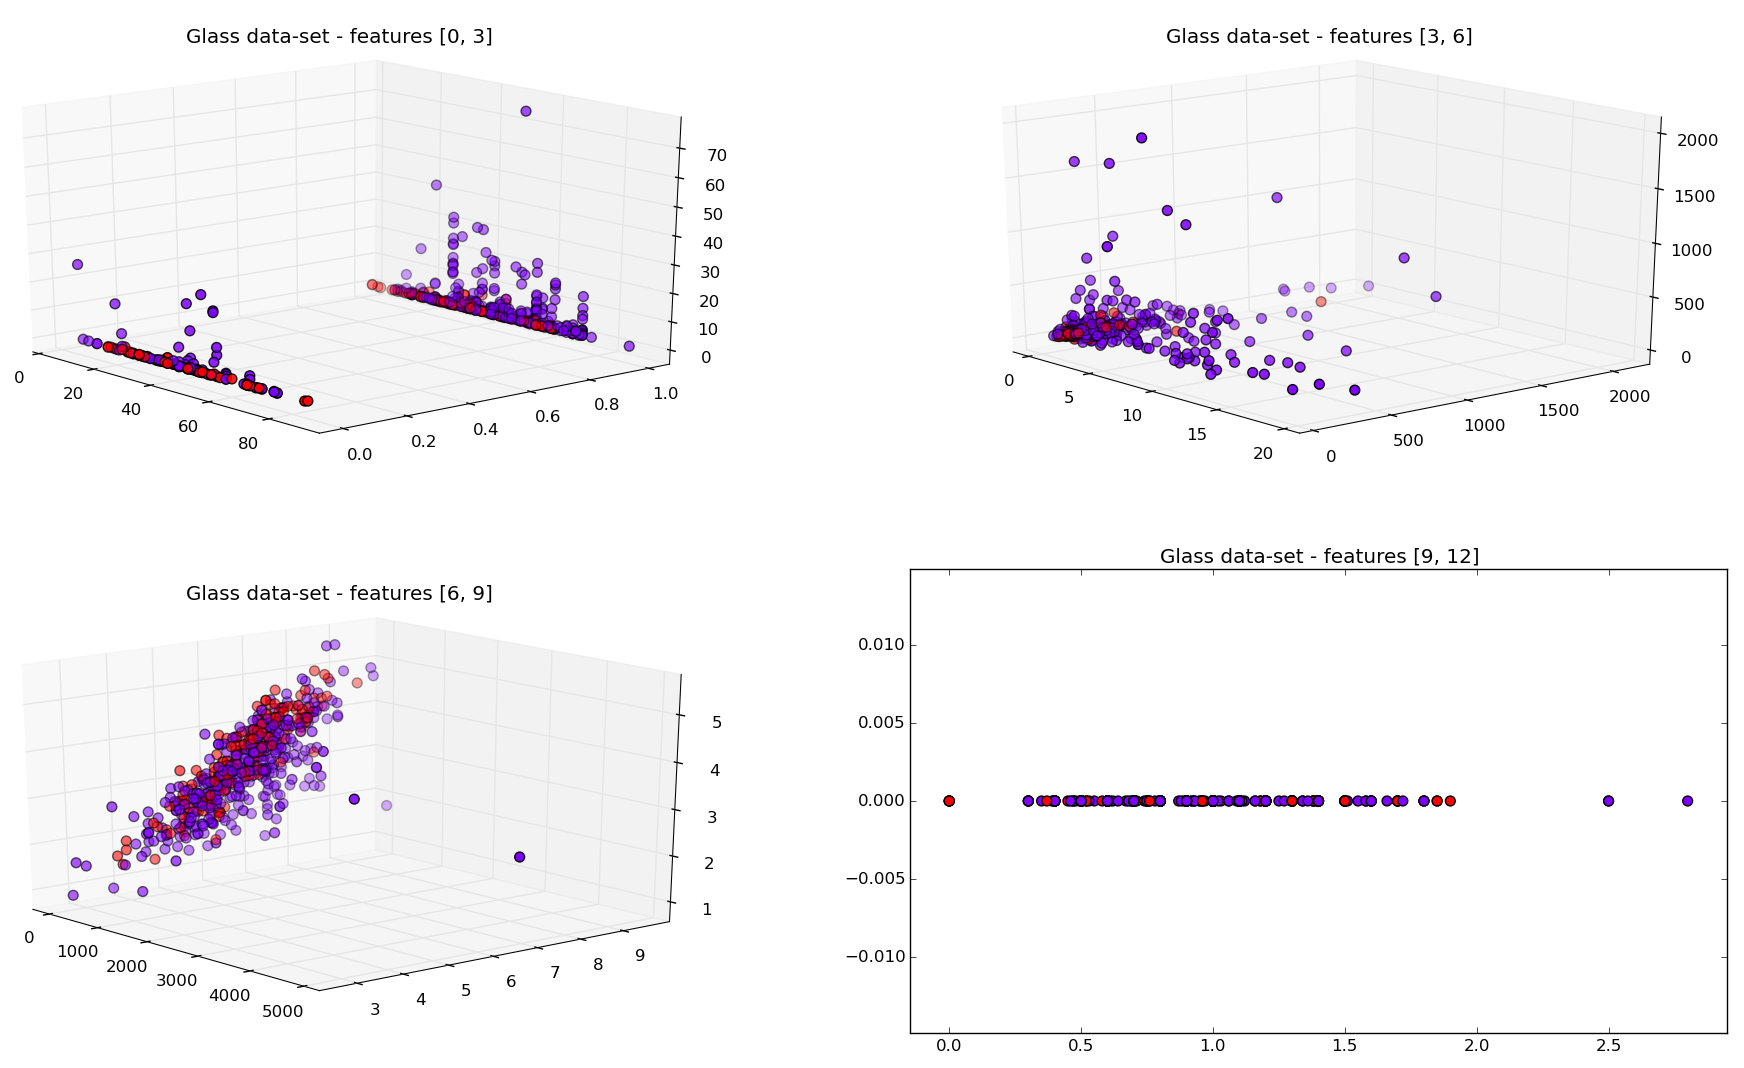
\includegraphics[scale=.3]{experiments/3_1_2_displaying_ilpd}
	\caption{The data set ILPD mapped onto $\mathbb{R}^n$, where each of its features is an axis, except for $S \coloneqq \{1, 2\}$, which was represented by the vertices' colors.}
	\label{fig:disp_ilpd}
\end{figure}

Considering the many graphs required to display the data set, it is quite difficult to identify a plausible distribution for ILPD. We define here our first encouragement towards the study of dimensionality reduction: the identification of the most significant features and plotting of those might result on simpler and more intuitive representations.

\subsubsection{Modern Problems and Applications}

Differently from Iris flower or ILPD data set, data sets associated with modern problems are often very dense, i.e., data sets containing many samples and/or features. Although the high number of samples is essentially benefic, a high number of features might be irrelevant or even unconstructive to the learning process. \cite{cay2005}

\begin{table}[H]
	\begin{tabular}{ c | *{4}{|c}| }
		& A & B & … & AAAV \\ \hline
		1 & 0.0111486888670454 & -0.01541263850539861 & … & 0.007440367302352156 \\
		2 & 0.03016080450207878 & 0.1772161342899135 & … & 0.01309011094914101 \\
		… & … & … & … & … \\
		8200 & 0.02680808496910305 & -0.0320375843317954 & … & 0.1772161342899135 \\
	\end{tabular}

	\caption{A data set with 8200 samples and 100 features.}
\end{table}

In many cases, there are indicatives that the data set lie near a lower-dimensional manifold embedded in the $\mathbb{R}^n$. \cite{gho2006} For the data set above, in special, the $\mathbb{R}^{100}$. A second encouragement can then be set: it is possible that the data set might be shrunk by combining similar (linearly dependent) features or eliminating the ones that poorly contribute towards the learning process. In order to do this, one must be able to qualify the “contribution” of each feature or even identify dependencies between features.

\subsection{Probability Theory}
\subsubsection{Feature Standardization}
Many of the methods ahead will require the data set to be centered in the origin. To center a data set $X$, we build a data set $X'$ s.t. each column has zero mean and it is contracted by its standard deviation:
$$X'_{.j} = \frac{X_{.j} - \mu}{\sigma} \textnormal{, where}$$
\begin{enumerate}
	\item $X_{.j}$ is the j-th column of the matrix $X$.
	\item $\mu$ is the mean of $X_{.j}$.
	\item $\sigma$ is the standard deviation of $X_{.j}$.
\end{enumerate}

\subsubsection{Centering Matrix}
The symmetric matrix $H$ is named the \textbf{centering matrix} when the multiplication of it by a vector $X$ produces the same effect of subtracting the mean of the components from each component of $X$. $H$ is defined as:
$$
H = I_n - \frac{1}{n}\textbf{11}^T \textnormal{, where:}
$$
\begin{enumerate}
	\item $I_n$ is the identity matrix of order $n$.
	\item $\textbf{1}$ is the column vector of 1's.
\end{enumerate}

\subsubsection{Variance}
Variance is the measure which describes how far the samples in a given set X vary. For this work scope, will consider only discrete probabilities. That is, if $X$ represents a variate with known distribution $P(x)$, where $\sum P(x) = 1, \forall x \in X$ and population mean $\mu$, then
$$
var(X) = \frac{1}{n} (X-\mu) \cdot (X-\mu) = \frac{1}{n} \sum (x - \mu)^2, \forall x \in X
$$

\begin{remark}
	If $var(X) = 0$, then it is easy to assert that all variables in $X$ assume the exact same value by using the elementary properties of the inner product.
\end{remark}

\begin{example}
	If $X=\{1, 2, -2, 4\}$ and $\mu = \frac{1}{4} \sum X_i = \frac{1+2-2+4}{4} = 1.25$, then
	\begin{align*}
	var(X) &= \frac{1}{4} \sum (X_i - \mu)^2 \\
	&= \frac{(1-1.25)^2 + (2-1.25)^2 + (-2-1.25)^2 + (4-1.25)^2}{4} \\
	&= 4.6875
	\end{align*}
\end{example}

\begin{example}
	The variance of the Sepal length feature in the Iris flower data set can be calculated as:
	\begin{align*}
	var(X) &= \frac{1}{150} \sum (X_i - \mu)^2 \\
	&= \frac{1}{150} [(5.1-5.84)^2 + (4.9-5.84)^2 + \cdots + (5.9-5.84)^2] \\
	&= \frac{102.17}{150} = .681122
	\end{align*}
\end{example}

\subsubsection{Covariance}

The covariance measures the variance of two random variates in respect to each other. Formally, if $X$ and $Y$ are two given random variates with known mean population distribution $\mu_X$ and $\mu_Y$, respectively, then
$$\sigma(X, Y) = \frac{1}{n} (X - \mu_X) \cdot (Y - \mu_Y) $$

Simply putting, the covariance of two random variables $X$ and $Y$ can be interpreted as one of the following behaviors:
$$
\sigma(X,Y) = \begin{cases}
\sigma_{xy} > 0 \implies \textnormal{X tends to increase as Y increases.}\\
\sigma_{xy} < 0 \implies \textnormal{X tends to increase as Y decreases.}\\
\sigma_{xy} = 0 \implies \textnormal{X and Y are completely unrelated.}
\end{cases}
$$

\begin{remark}
	For a random variate $X$, $var(X) = \sigma(X, X)$.
\end{remark}

\paragraph{Covariance Matrix of Features in a Centered Data Set}

Let $D$ be a data set, $H$ the centering matrix and $HD_{\_i}$ the {\em i-th} feature column of the centered data set $HD$, the covariance between each one of its features can be represented by the matrix:
\begin{align*}
\Sigma &= [\sigma_{xy}]_{n \times n} \\
&= \begin{bmatrix}
\sigma(HD_{\_0}, HD_{\_0}) & \sigma(HD_{\_0}, HD_{\_1}) & \cdots & \sigma(HD_{\_0}, HD_{\_n-1}) \\
\sigma(HD_{\_1}, HD_{\_0}) & \sigma(HD_{\_1}, HD_{\_1}) & & \sigma(HD_{\_1}, HD_{\_n-1}) \\
\vdots &&& \vdots \\
\sigma(HD_{\_n-1}, HD_{\_0}) & \sigma(HD_{\_n-1}, HD_{\_1}) & \cdots & \sigma(HD_{\_n-1}, D_{\_n-1})
\end{bmatrix} \\
&= \frac{1}{n} (HD)^T HD \\
&= \frac{1}{n} D^T H^T H D \\
 &= \frac{1}{n} D^T H D
\end{align*}

Where $H$ is the \textbf{centering matrix}.

\subsubsection{Correlation}

``The correlation is a measure of the direction and strength of a linear relationship among variables."

Let $X$ and $Y$ be two random variables, $r(X, Y)$, i.e., the correlation between $X$ and $Y$ is defined as:
\begin{align*}
	r(X, Y) = \frac{\sigma(X, Y)}{\sigma_X \sigma_Y},
\end{align*}

where $\sigma_X$ and $\sigma_Y$ are the standard deviations of the variables $X$ and $Y$, respectively.

\begin{remark}
	If $X$ and $Y$ are two random variables and $\sigma(X, Y) = 1$, $X=Y$.
\end{remark}

\paragraph{Correlation Matrix of Features in a Centered Data Set}

Let $D$ be a data set, $H$ the centering matrix and $HD_{\_i}$ the {\em i-th} feature column of the centered data set $HD$. The correlation between each one of its features can be represented by the matrix:
\begin{align*}
	corr(D) &= \begin{bmatrix}
		1 & \frac{\sigma(HD_{\_0}, HD_{\_1})}{\sigma_{HD_{\_0}} \sigma_{HD_{\_1}}} & \cdots & \frac{\sigma(HD_{\_0}, HD_{\_n-1})}{\sigma_{HD_{\_0}} \sigma_{HD_{\_n-1}}} \\
		\frac{\sigma(HD_{\_1}, HD_{\_0})}{\sigma_{HD_{\_1}} \sigma_{HD_{\_0}}} & 1 & \cdots & \frac{\sigma(HD_{\_1}, HD_{\_n-1})}{\sigma_{HD_{\_1}} \sigma_{HD_{\_n-1}}} \\
		\vdots & \vdots && \vdots \\
		\frac{\sigma(HD_{\_n-1}, HD_{\_0})}{\sigma_{HD_{\_n-1}} \sigma_{HD_{\_0}}} & \frac{\sigma(HD_{\_n-1}, HD_{\_1})}{\sigma_{HD_{\_n-1}} \sigma_{HD_{\_1}}} & \cdots & 1
	\end{bmatrix}
\end{align*}

\subsection{Numerical Analysis}
\subsubsection{Eigenvalues and Eigenvectors of a Matrix}

Given a matrix $A \ne 0 \in \mathbb{R}^{2n}$, a vector $v \in \mathbb{R}^n$ is said to be an \textbf{eigenvector} of $A$ if the multiplication $Av$ does not change the direction of $v$; that is:
$$\exists \lambda \in \mathbb{R} \mid Av = \lambda v \textnormal{, where}$$
$\lambda$ is the \textbf{eigenvalue} associated to the eigenvector $v$.

\subsubsection{Spectral Decomposition of a Matrix}

If $[M]_{n\times n}$ is a symmetric matrix of rank $n$ and admits $n$ pairs of eigenvalues $\lambda$ and eigenvectors $[V]_{n\times n} = [v_0, v_1, v_2, ..., v_{n-1}]$, such that $V^TV = 1$, then
$$MV = V \lambda$$

$\lambda = diag(\sigma_0, \sigma_1, ..., \sigma_{n-1})$ is the diagonal matrix, where $\sigma_i$ is the eigenvalue associated to the eigenvector $v_i$. \cite{cox2001} Furthermore, $V$'s columns are linear independent, hence $V$ is invertible.
\begin{align*}
	MV &= V \lambda \\
	MVV^T &= V \lambda V^T \\
	M &= V \lambda V^T
\end{align*}

\subsubsection{Singular Value Decomposition}
\label{sec:svd}
If $M \in \mathbb{R}^{m \times n}$, then $\exists U \in \mathbb{R}^{m \times m}, V \in \mathbb{R}^{n \times n}$ and $\Sigma =  diag(\sigma_0, \dots, \sigma_{n-1})$ conditioned to $\sigma_i \ge \sigma_{i+1} \ge 0, \forall \sigma \in [0, n)$ s.t. \cite{gan2008}
$$M = U\Sigma V^T$$

\begin{theorem}
	\label{th:svd-aat}
	If $A = U \Sigma V^T$, $AA^T = U \Sigma^2 U$ and $A^TA = V \Sigma^2 V$.
\end{theorem}
\textbf{Proof}
\begin{align*}
	A^TA &= (U\Sigma V^T)^T(U\Sigma V^T) \\
	&= V \Sigma^T U^T U \Sigma V^T \\
	&= V \Sigma \Sigma V^T \\
	&= V \Sigma^2 V^T
\end{align*}

Proving $AA^T = U \Sigma^2 U^T$ is analogous to the above.

\subsection{Topology}
\subsubsection{Manifolds}

Intuitively, n-dimensional topological manifolds are sets that are ``locally Euclidean". \cite{lee2009} In other words, they can be decomposed into sub sets that can be mapped to the $\mathbb{R}^n$.

Formally, a set $M$ is said to be a \textbf{n-dimensional topological manifold} $\iff M$ is a paracompact Hausdorff topological space $\mid \forall p \in M, p \in U_p$, where $U_p$ is an open set that is homeomorphic to an open set $V_p$ of the Euclidean space $\mathbb{R}^n$. \cite{lee2009}

From here, we will use the word manifold to refer to the n-dimensional topological manifold.

\paragraph{Charts}
The pair $(U_i, \phi_i)$ is called a \textbf{coordinate chart} or \textbf{chart} on $M$ if $U \in M$ and $\phi_i$ is a \textbf{homeomorphism} such that $\phi_i(U_i) = V_i \subseteq \mathbb{R}^n$ \cite{lee2012}.

\paragraph{Atlas}

A set $A = \{(U_i, \phi_i)\}_{i \in A}$ is said to be an \textbf{atlas} on a manifold $M$ if $\cup_{i \in A} U_i = M$ \cite{lee2012}.

\begin{example}
	The $\mathbb{R}^n$ is, directly, a manifold.
\end{example}

\begin{example}
	A n-dimensional sphere is a manifold. Earth, in special, is a 3-dimensional sphere and its stereographic projection is its mapping to the $\mathbb{R}^2$. \cite{stereo_proj}

	\begin{figure}[H]
		\centering
		\captionsetup{justification=centering}

		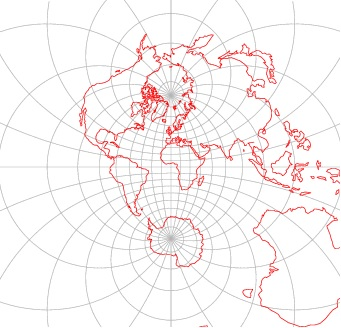
\includegraphics[scale=.8]{stereo_earth}
		\caption{Stereographic projection applied to Earth.}
		\label{fig:stereographic_earth}
	\end{figure}
\end{example}

\subsection{Graph Theory}
\subsubsection{Graphs}

Let $G$ be the pair $(X, U)$. $G$ is defined as a \textbf{graph}, \cite{berge1973} where
\begin{enumerate}
	\item $X$ is a set of objects called \textbf{vertices}.
	\item $U$ is a family of elements $u_i \in X\times X$ called arcs.
\end{enumerate}

\paragraph{Basic Concepts \cite{berge1973}}
\begin{description}
	\item[Multiplicity] If $G=(X, U)$ and $(x, y) \in X\times X$, the multiplicity $m_g^+(x, y)$ of $x, y$ is defined to be the number of arcs with initial endpoint $x$ and terminal endpoint $y$. Furthermore:
	\begin{enumerate}
		\item $m_G^-(x, y) = m_G^+(y, x)$
		\item $m_G(x, y) = m_G^+(x, y) + m_G^-(x, y)$
	\end{enumerate}

	\item[Degree] If $G=(X, U)$ is a graph and $x\in X$, the degree $d(x)$ of $x$ is defined \cite{may1972} as
	$d(x) = 2n_s  + n_n$, where $n_s$ is the number of arcs self-incident at $x$ (i.e., $\{(x, x)\}$) and $n_n$ is the number of arcs incident at $x$.

	\item[Adjacency Matrix] If $G=(X, U), X=\{x_1, x_2, \dots, x_n \}$, define the adjacency matrix $A=[a_{ij}]_{n\times n}$ associated with graph $G$, where $a_{ij} = m_G^+(x_i, x_j)$.
\end{description}

\paragraph{Further Specifications}

\begin{description}
	\item[Undirected graph] ``All graphs are directed, but sometimes the direction need not be specified \cite{berge1973}".

	Let $G=(X, U)$ be a graph and $u_k \in U \mid u_k=(a, b)$. The element $e_i=[a, b]$ can be defined as the \textbf{edge} that links $a$ to $b$ without specifying direction. Finally, define the \textbf{undirected graph} $H$ as $(X, E)$, where $E=\{e_i\}$ is the set of edges created from $U$.

	Figure \ref{fig:graph} shows the graph \textbf{Les Miserables}, where each node is a character and each arc links two characters that have shared stage at some point during the play.

	\begin{figure}[H]
		\centering
		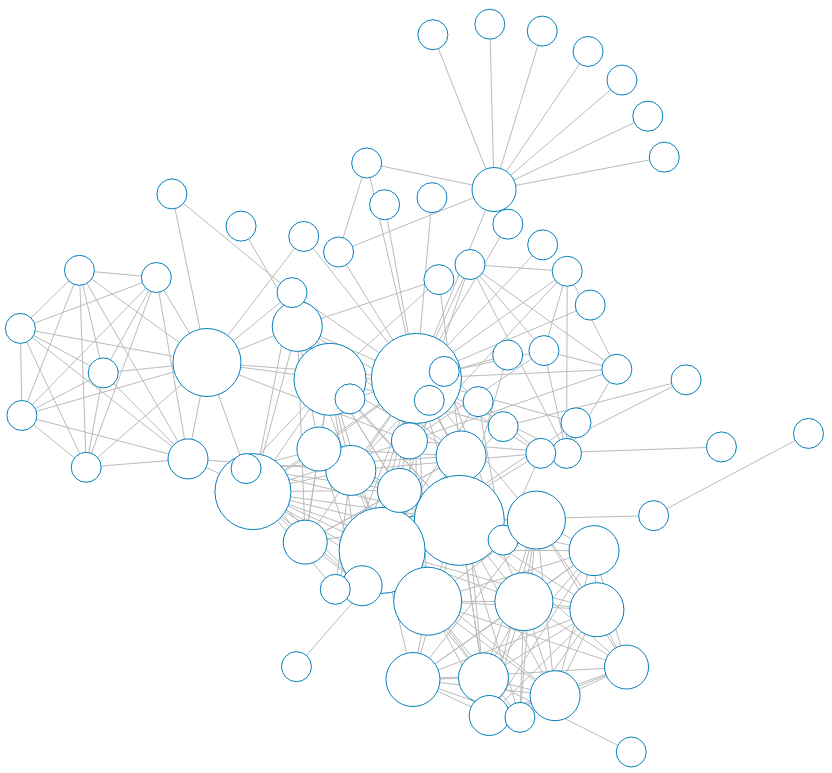
\includegraphics[width=.5\linewidth]{graph}
		\caption{The \textbf{Les Miserables} graph.}
		\label{fig:graph}
	\end{figure}

	\item[Complete graph] A graph $G=(X, U)$ is said to be complete if
	$$\forall (x, y)\in X, x\ne y, m_G(x, y) \ge 1$$

	\begin{remark}
		Let $G=(X, U), G_1=(X, E)$ and $n=|X|$. $G$ is called the complete graph $K_n$ if
		$$\forall (x, y)\in X, \exists e \in E \mid e=[x, y]$$
	\end{remark}

	\item[Weighted graph] Let $G=(X, U)$ be a graph and $w\colon U \to \mathbb{R} \mid w(u) = w_u$ be the weighted associated with arc $u$. $G$ is said to be a weighted graph.

	\item[Euclidean graph] If $G=(X, U)$ and $W=\{w_u, \forall u\in U\}\subset \mathbb{R}$, $G$ is said to be an euclidean graph if $w_u$ corresponds to the euclidean distance between the vertices connected by $u$ in a specified embedding.

	\item[Tree] Let $G$ be the graph $(V, E)$ such that $G$ is connected and admits no cycles. $G$ is  said to be a \textbf{tree} \cite{berge1973}.

	\begin{figure}[H]
		\centering
		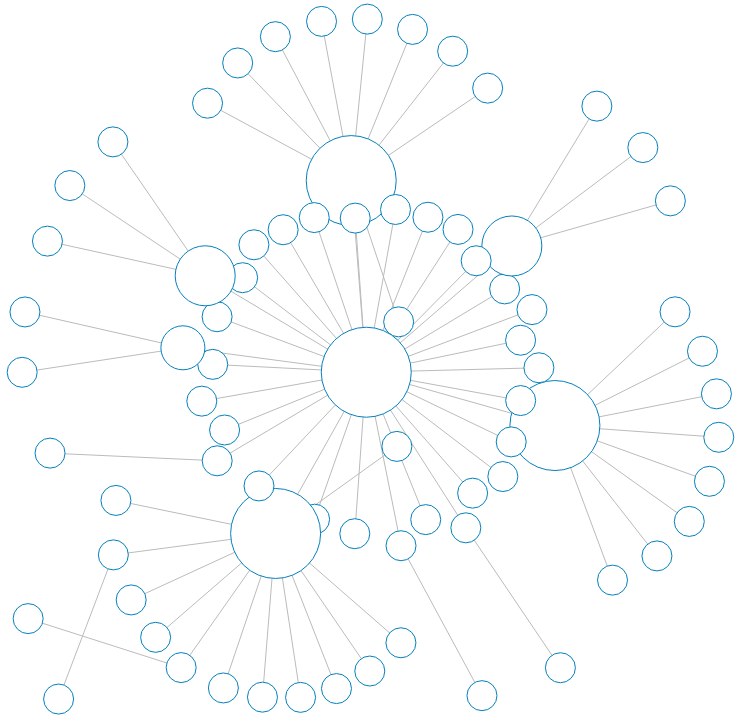
\includegraphics[width=.4\linewidth]{tree}
		\captionsetup{justification=centering}
		\caption{A tree extracted (a subgraph) from the \textbf{Les Miserables} graph.}
		\label{tree}
	\end{figure}
\end{description}

\subsubsection{Related Problems}

\paragraph{Nearest-Neighbor Search}

Let $G = (X, U)$ be a weighted graph, where $ \forall u \in U, \exists w_u \in \mathbb{R}$, i.e., the weight or \textbf{length} of the arc $u$, and $n\colon U \to \{0, 1\}$ a definition of \textbf{nearness} in $G$. The nearest-neighbor search is a optimization problem that consists of finding a subgraph $H = (X, F \subseteq U) \mid f \in F \iff n(f) = 1$.

\subparagraph{A Generic Algorithm for NN Search}
\begin{enumerate}
	\item $F_x \coloneqq \emptyset, \forall x \in X$
	\item $F_x \coloneqq F_x \bigcup_{\forall p \in U_x} \begin{cases}
	\{p\}, \text{if } n(p) = 1 \\
	\emptyset, \text{if } n(p) = 0 \\
	\end{cases}$
	\item $H \coloneqq (X, F), F = \cup_{x\in X} F_x$
\end{enumerate}

Let's consider two (between many)  specifications of this algorithm:

\begin{description}
	\item[K-Nearest Neighbor Search (K-NN)] Fixed $k \in \mathbb{N}$ and $U_x \subseteq U$, where $U_x$ is the set of all arcs with $x$ as initial endpoint, define:

	\begin{align*}
	n(u_x) &\coloneqq \begin{cases}
		1, \text{if }  w_{u_x} \le w_p, \forall p \in U_x - F_x \text{ and } |F_x| \le k \\
		0, \text{otherwise.} \\
		\end{cases}
	\end{align*}

	\item[$\epsilon$-Nearest Neighbor ($\epsilon$-NN)] Fixed $\epsilon \in\mathbb{R}$, define:
	\begin{align*}
		n(f) &\coloneqq \begin{cases}
			1, \text{if } w_f \le \epsilon \\
			0, \text{otherwise} \\
		\end{cases}
	\end{align*}
\end{description}

\begin{example}
	If $k=1$ and $\epsilon=60$, the graph $G$, the sub-graph $H$ found from K-Nearest neighbor algorithm and the sub-graph $I$ found from the $\epsilon$-Nearest neighbor are defined as follows:
	\begin{figure}[H]
		\begin{subfigure}{.33\linewidth}
			\centering
			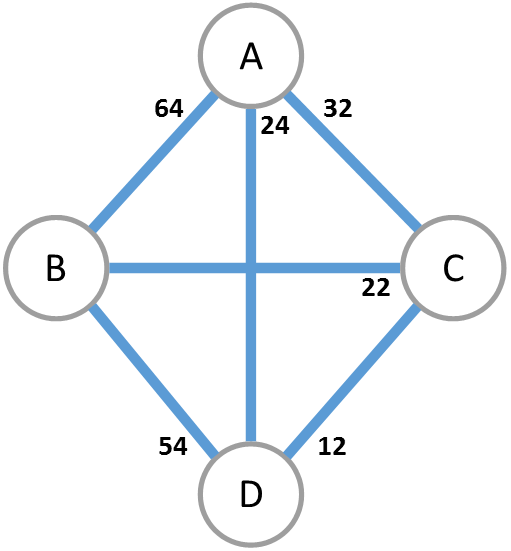
\includegraphics[width=.8\linewidth]{example-graph}
			\caption{$G$}
			\label{fig:example-graph}
		\end{subfigure}%
		\begin{subfigure}{.33\linewidth}
			\centering
			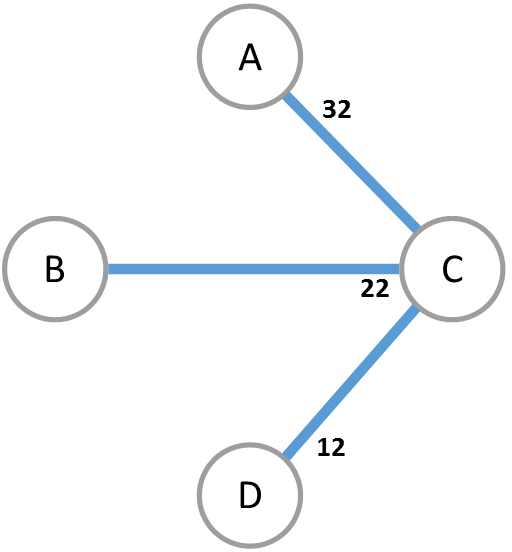
\includegraphics[width=.8\linewidth]{example-graph-nn}
			\caption{$H$}
			\label{fig:example-graph-nn}
		\end{subfigure}%
		\begin{subfigure}{.33\linewidth}
			\centering
			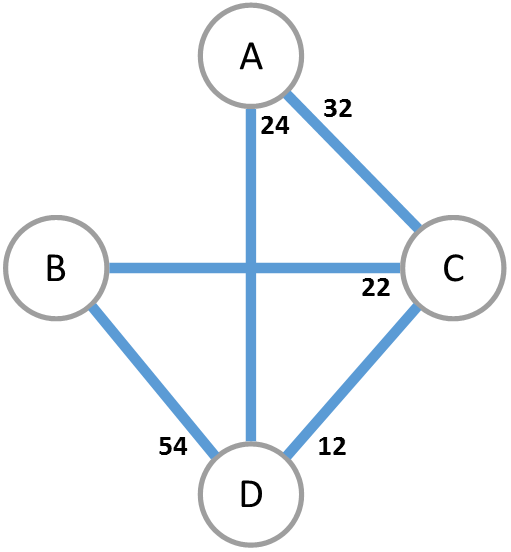
\includegraphics[width=.8\linewidth]{example-graph-en}
			\caption{$I$}
			\label{fig:example-graph-en}
		\end{subfigure}
	\end{figure}
\end{example}

\paragraph{Shortest-path Problem \cite{cor2011}}

Let $G=(X, U)$ be a weighted graph, a path $p(x, y)=(u_0, u_1, u_2, \dots, u_{p-2}, u_{p-1}, u_{p}) \mid u_0 = (x, \_), u_p = (\_, y), u_i \in U, \forall i \in [0, p]$, and the weight of $p$ be given by $w(p) = \sum_i^p w(u_i)$. The shortest-path weight between two vertices $x$ and $y$ is defined as:
\begin{align*}
	\sigma(x, y) = \begin{cases}
		\min \{w(p(x, y))\}, \text{ if $p(x, y)$ exists}, \\
		\infty, \text{ otherwise.}
	\end{cases}
\end{align*}

while $p(x, y)$ is the \textbf{shortest path} from $x$ to $y$.

The shortest-path between a vertex $x_0 \in X$ and all other vertices can be expressed by the tree $S=(X, F), F \subseteq U$, denominated \textbf{shortest-path tree}.

\subparagraph{Dijkstra's Algorithm \cite{cor2011}}

\begin{example}
	Let G be the weighted graph as defined in figure \ref{fig:spa-graph}. The shortest-path between $A$ and all other vertices is described by the tree $S$ illustrated in figure \ref{fig:spa-tree}.

	\begin{figure}[H]
		\centering
		\begin{subfigure}{.4\linewidth}
			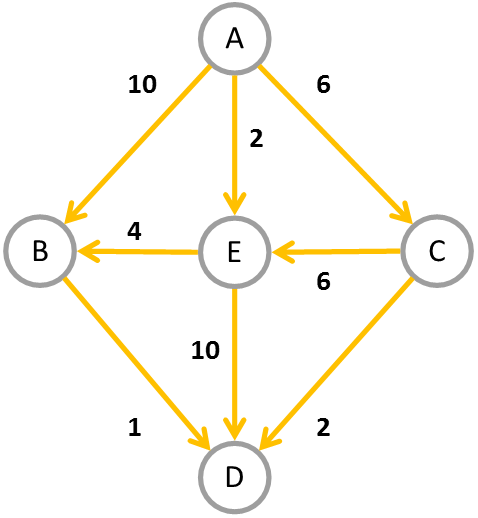
\includegraphics[width=\linewidth]{spa-graph}
			\captionsetup{justification=centering}
			\caption{The weighted graph $G$.}
			\label{fig:spa-graph}
		\end{subfigure}
		\begin{subfigure}{.4\linewidth}
			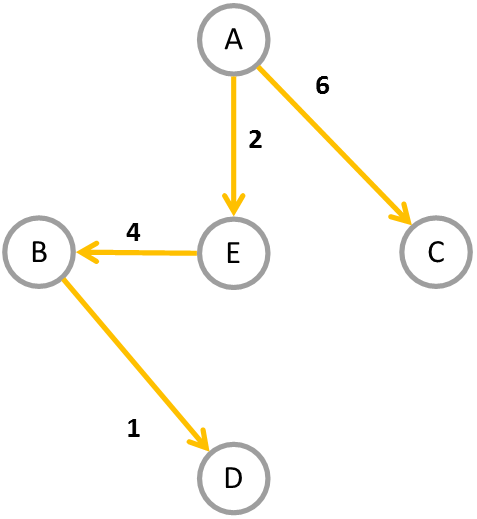
\includegraphics[width=\linewidth]{spa-tree}
			\captionsetup{justification=centering}
			\caption{The shortest-path tree $S$.}
			\label{fig:spa-tree}
		\end{subfigure}
	\end{figure}
\end{example}

\subsection{Machine Learning}
“Learning is the improvement of performance is some environment through the acquisition of knowledge resulting from experience in that environment." \cite{pat1996}

“Machine learning is the area in Computer Science that has as goal the projection and implementation of machines that have the ability to learn autonomously”. \cite{hot2009} In other words, the creation of machines that are able to recognize patterns in an environment and interpret those using concepts related to artificial intelligence. Such interpretation can create a model which might eventually be used to predict new patterns, take actions and/or solve domain problems.

\subsubsection{Machine Learning Algorithms}

Based on how the learning phase of a problem is, most of the ML algorithms may be divided into one of the following categories:

\begin{description}
	\item[Supervised] A direct feedback is presented during the learning phase. \cite{pat1996} For the instances where the ME problem relies on a data set, the learning task uses the labeled training samples (i.e., samples that present the \textbf{target feature}) to synthesize the model that attempts to generalize the relationship between the feature vectors and the target variable. \cite{awa2015}

	\item[Unsupervised] Infer hidden structures from the data set without direct feedback, such as known labels for the samples. \cite{awa2015}

	\item[Semi-supervised] Most commonly, it is given by the extension of either supervised or unsupervised learning to include the other paradigm, resulting in a combination of both. \cite{zhu2009}

	\item[Reinforcement] Through iterative exploration, the learner is positively or negatively reinforced for its actions. The learner's goal is, ultimately, maximize the cumulative reward gained. \cite{awa2015}
\end{description}

\paragraph{Support Vector Machine: An Example of Supervised Learning}

The Support Vector Machine algorithm (i.e., SVM) is a is a powerful tool, often used in classification problems.

Intuitively, the SVM algorithm attempts to find a hyperplane that separates the samples in a data set into two different groups: positives and negatives. Furthermore, the hyperplane is placed such that the distance between the \textbf{support vectors} (the closest samples) and it are maximized.

\begin{figure}[H]
	\centering
	\captionsetup{justification=centering}

	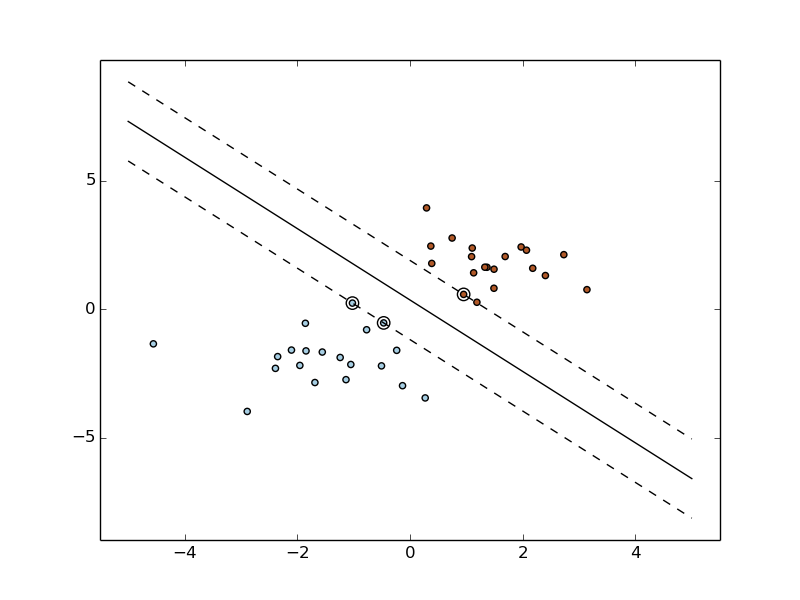
\includegraphics[scale=.5]{svm_margin}
	\caption{A SVM classifier projecting a hyperplane that perfectly separates two classes of samples. \cite{sksvm}}
	\label{fig:svmmargin}
\end{figure}

More elaborately, given any linearly separable data set $X$ containing samples from two distinguished classes $\{-1, +1\}$, consider the vector $w$ a hyperplane $d = \{x \mid w \cdot x + b = 0\}$ (represented in fig. \ref{fig:svmmargin} by the contiguous line) s.t.
$$\text{\textbf{decision rule}} \begin{cases}
	w \cdot u +b \geq 0 \implies y_u=+1\\
	w \cdot u +b < 0 \implies y_u=-1\\
\end{cases}$$

To prevent samples from falling into the margin or being misclassified, \cite{wessvmdef} reinforce that for any positive sample $x_+$, $w \cdot x_+ +b \geq 1$. Similarly for $x_-$ samples, $w \cdot x_- +b \leq 1$. These both constraints can be expressed as
\begin{equation} \label{svmconst}
y_i(w \cdot x_i +b) -1 \geq 0
\end{equation}

Notice that $y_i(w \cdot x_i +b) -1 = 0 \iff x_i $ is a \textbf{support vector}.

The width (the distance between the two margins) of the street is the vector $(x_+^0 -x_-^0)$ projected onto the vector $w$, where $x_-^0$ is a positive support vector and $x_+^0$ is a negative one.
\begin{equation} \label{eq:eqsvmwidth}
\begin{split}
width &= (x_+^0 - x_-^0) \cdot \frac{w}{\|w\|} \\
      &=\frac{x_+^0 \cdot w - x_-^0 \cdot w}{\|w\|} \\
      &=\frac{1-b - (-1-b)}{\|w\|} = \frac{2}{\|w\|}
\end{split}
\end{equation}

As the goal is to maximize the width, while still respecting the constraint (\ref{svmconst}).
\begin{equation} \label{eq:svmminw}
	\max width = \max \frac{2}{\|w\|} \equiv \min \frac{1}{2} \|w\|^2
\end{equation}

Which can be solved using standard quadratic programming.

\paragraph{SVM for non-separable data sets (soft margins)}

To deal with non-separable data sets, it is possible to introduce the variables $\xi_i$, \cite{wessvmdef} which represent a trade-off between maximum margin/distance of the misclassified samples from the decision boundary.
$$\min \frac{1}{2} \|w\|^2 + C \sum_{1}^{m}\xi_i \text{, constrained to:}$$
$$y_i(w \cdot x_i +b) \geq 1- \xi_i, \xi_i \geq 0$$

Such trade-off can be adjusted through the parameter $C$. Notice that small values for $C$ might result in misclassification, whereas high values can produce overfitting.

\paragraph{Dependency over the dot product}

Equation \ref{eq:svmminw} does not explicitly illustrates how the model generated depents on the dot product between the training samples. The implications of such fact will be discussed in the next section. For now, let us convert \ref{eq:svmminw} to its dual form. By the Lagrange multipliers method: \cite{mitsvm}
\begin{align} \label{eq:svmlag1}
	L &= \frac{1}{2}\|w\|^2 - \sum \alpha_i[y_i(w \cdot x_i +b) -1] \\
	\label{svmlag2}
	\frac{\partial L}{\partial w} &= w -\sum\alpha_i y_i x_i = 0 \implies w = \sum\alpha_i y_i x_i \\
	\label{svmlag3}
	\frac{\partial L}{\partial b} &= -\sum\alpha_i y_i = 0 \implies \sum\alpha_i y_i = 0
\end{align}

Applying (\ref{svmlag2}) and (\ref{svmlag3}) on (\ref{eq:svmlag1}), our problem of minimizing (\ref{eq:svmminw}) constrained by (\ref{svmconst}) becomes maximizing $L$, subject to (\ref{svmlag3}):
\begin{gather*}
L = \frac{1}{2}\sum\alpha_i y_i x_i \cdot \sum\alpha_j y_j x_j
- \sum \alpha_i y_i x_i \cdot \sum \alpha_j y_j x_j
- \sum \alpha_i y_i b + \sum \alpha_i \\
= \sum\alpha_i -\frac{1}{2}\sum\sum\alpha_i\alpha_j y_i y_j (x_i \cdot x_j)
\end{gather*}

$w$ and $b$ can easily be found from (\ref{svmlag2}) and $\alpha_i[y_i(w \cdot x_i + b) - 1] = 0$ (for any $i \mid \alpha_i \ne 0$), respectively.

Now, as we finally plug (\ref{svmlag2}) back into our decision rule, it becomes clear that both training and prediction phases depend only on the dot product between the sample vectors: \cite{mitsvm}

$$\text{\textbf{decision rule}} \begin{cases}
	\sum\alpha_i y_i x_i \cdot u +b \geq 0 \implies y_u=+1\\
	\sum\alpha_i y_i x_i \cdot u +b < 0 \implies y_u=-1\\
\end{cases}$$

\paragraph{Kernel functions}

"The kernel function represent the dot product of both vectors projected onto the new space". \cite{mitsvm}

Some data sets are not linearly separable, as mentioned in a few sections above. They can, however, be projected to a different vector space, where they hopefully will be. To achieve this, a transformation $\phi$ is applied on both vectors. The dot product between those is then calculated in the new space and the value is used during training (the maximizing $L$) and prediction (the decision rule):
\begin{gather*}
L = \sum\alpha_i -\frac{1}{2}\sum\sum\alpha_i\alpha_j y_i y_j \phi(x_i) \cdot \phi(x_j)
\end{gather*}

\begin{remark}
	Practically, Let $k: (\mathbb{R}^n, \mathbb{R}^n) \rightarrow \mathbb{R} \mid k(u, v) = \phi(u) \cdot \phi(v)$,
	\begin{gather*}
	L = \sum\alpha_i -\frac{1}{2}\sum\sum\alpha_i\alpha_j y_i y_j k(x_i, x_j)
	\end{gather*}
	
	Which entails, given a known function $k$, there is no need to explicitly know which are the projections of $x_i$ and $x_j$ onto the new vector space. This is commonly known as the \textbf{kernel trick}.
\end{remark}

$$\text{\textbf{decision rule}} \begin{cases}
\sum\alpha_i y_i k(x_i, u) +b \geq 0 \implies y_u=+1\\
\sum\alpha_i y_i k(x_i, u) +b < 0 \implies y_u=-1\\
\end{cases}$$

The figure bellow illustrates a non-linearly separable data set defined in the $\mathbb{R}$ being projected to the $\mathbb{R}^2$.

\begin{figure}[H]
	\centering
	\captionsetup{justification=centering}

	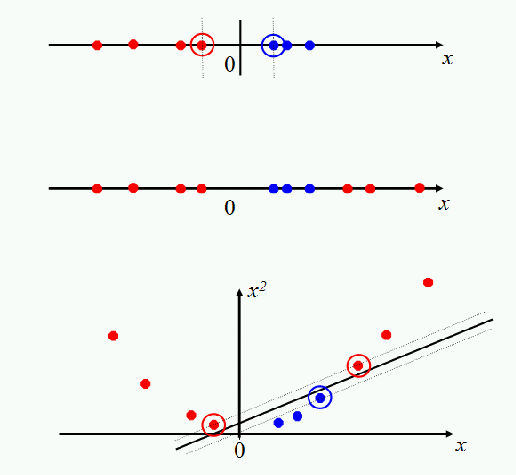
\includegraphics[scale=.4]{svm_kernel}
	\caption{Projection of samples from the $\mathbb{R}$ to the $\mathbb{R}^2$, allowing SVM to find a hyperplane that perfectly separates both classes. \cite{svmkernels}}
	\label{fig:svmkernel}
\end{figure}

Between many different kernels, two often used are the RBF: $\exp(-\frac{\|x -x'\|^2}{2\sigma^2})$ and the Polynomial: $(u^T v + c)^{d}$. \cite{svmkernels}

\subsubsection{Multi-class Classification}

Not all problems are binary. In classification, this reflects data sets that have their samples separated into more than two classes. The Iris flower data set is an example of this, when predicting the samples' {\em species}.

There are many different approaches for multi-class classification. \cite{rif2008} For the scope of this work, consider only the following:

\begin{description}
	\item[One-vs-All (OVA)] $n$ binary classifiers are built, where $n$ is also the number of classes in the data set. For the classifier $c^j, j \in [1, n]$, all samples of the $j$th class are taken as positive examples, at the same time that all the other samples are considered negative.

	If
	$$c^j(x) = \sum_{i=1}^{m} y_i \alpha_i^j x \cdot x_i + b$$

	Then positive values for $c^j(x)$ indicate that the sample $x$ belongs to the $j$th class. Additionally, greater $c^j(x)$ values imply on further distance from the hyperplane (i.e., $c^j(x)$ can also be interpreted as a \textbf{confidence value}) and the sample $x$ should be assigned to the class which holds greatest confidence. \cite{ovacj} Shortly, classification is given by
	$$ f(x) = \argmax_j{c^j(x)} $$
	\item[All-vs-All (AVA)] Also known as all-pairs or one-vs-one, a classifier $c_{ij}$ is built for each pair of classes $(i, j)$, resulting in a total of $n(n-1)$ classifiers. $c_{ij}$ responds with positive values for samples of the $i$th class and negative values for samples of the $j$th class. Classification can be done by simply counting the class most frequently associated with $x$:
	$$ f(x) = \argmax_i{\sum_{j=1}^{n} c_{ij}(x)} $$
	Or equivalently, but only using $\frac{n(n-1)}{2}$ classifiers,
	$$ f(x) = \argmax_i{\sum_{j=1}^{n} \frac{j-i}{|j-i|} c_{\min(i, j) \max(i, j)}(x)} $$
\end{description}

\subsubsection{Evaluating learners}

Machine Learning algorithms might be susceptible to data noise, incorrect configuration or even random factors, which would eventually decrease the generated model's accuracy. In order to evaluate this same accuracy, models are quite often tested after trained.

Considering that testing with the same data used for training will most likely produce unreliable results, a simple way to test a learner is to separate the labeled data set into two chunks, where the first is used for training. The second chunk is then be given to the learner, which attempts to predict the samples. Finally, the predictions made by the learner would be compared with the actual labels.

\paragraph{Confusion Matrix}

When testing classification models, one way to visualize the wrong predictions made by the learner is a confusion matrix, where the item $a_{ij}$ is the number of times that a sample of the class $i$ was classified as being of the class $j$.

\begin{table}[H]
	\centering
	\begin{tabular}{ |c || *{4}{c|} }
		\hline
           &   a &   b &   c &   d \\\hline\hline
		a & 12 &   3 &   2 &   0 \\
		b &   7 & 12 &   2 &   4 \\
		c &   0 &   4 & 54 &   8 \\
		d &   6 &   0 &   1 & 23 \\\hline
	\end{tabular}

	\caption{Example of confusion matrix for a data-set with four different classes.}
\end{table}

Naturally, a diagonal matrix represents that all samples of the class $i$ were classified as $i$, which is the best possible outcome (no errors).

\paragraph{Cross Validation}

Sometimes (for example, when the data set does not have too many samples), partitioning of the data set into subsets might be benign to the learning process, as the model will be constructed only considering a small, random portion of the samples. This event is known as \textbf{underfitting}.

When $k$-fold cross-validating, \cite{crossvalid} the data set can be partitioned into $k$ folds. For each fold $k_i$, a model is trained with all folds, except for $k_i$. The model is then tested over $k_i$. Finally, the score reported by the cross-validation method is the average accuracy when testing over all folds.

\paragraph{Grid Search}

Machine Learning algorithms may require specific parameters to run. For instance, SVM requires $C$ and which $kernel$ it should use. Additionally, kernels might require their own parameters. As these parameters strongly affect how the generated model will be, one cannot choose them arbitrarily.

Grid Search is a traditional method used to find the parameters that optimize the generalization of learning model over a specific data set. \cite{gridsearch} Given a set of possible parameters, it will exhaustively search for the combination of those that generate the best outcome, which might be evaluated by a validation method such as cross-validation.

\subsubsection{Examples of Learning}

\paragraph{Coffee Selling Rate}

The figure bellow illustrates the distribution of coffee sales per time of the day in a particular coffee-shop. \cite{roh2015} Clearly being a regression problem, a machine learning algorithm must create a model that appropriately generalizes the distribution observed. Such model will eventually be used to predict the selling rate in the following days.

\begin{figure}[H]
	\centering
	\captionsetup{justification=centering}

	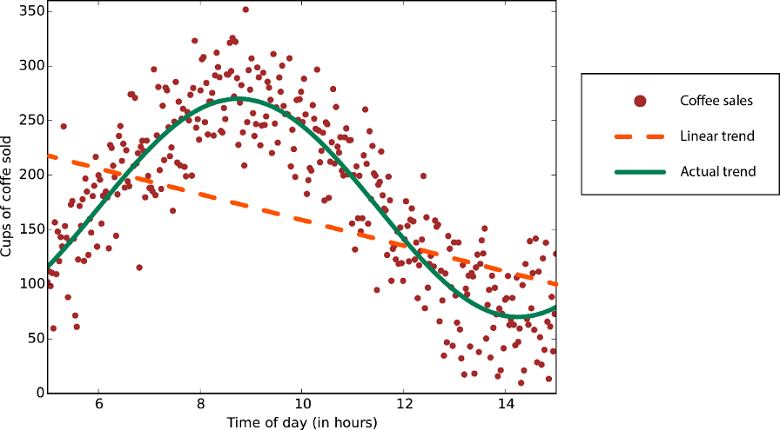
\includegraphics[scale=.6]{rohrer2015}
	\caption{graphic representation of a data set generalization by a linear (orange) and a nonlinear model (green).}
	\label{fig:rohrer2015}
\end{figure}

The orange line and the green arc represent two different models. The orange line, which represents the linear model, clearly does not generalize the data set appropriately, once it induces an error much larger than necessary. \cite{roh2015} The nonlinear model, i.e., the green arc, was capable of generalize the data inducing a smaller error.

\paragraph{Iris Flower}

Consider the Iris flower data set as defined in \ref{irisdataset}. In order to predict the feature {\em Species} of a given sample, one could train a Support Vector Machine classifier.

Through GridSearch, it was found that the SVM algorithm with $C=100$, $gamma=.01$ and $rbf$ kernel is capable of finding a model yielding .99\% accuracy. The samples misclassified during the test phase were represented by the confusion matrix bellow.

\begin{figure}[H]
	\centering
	\captionsetup{justification=centering}

	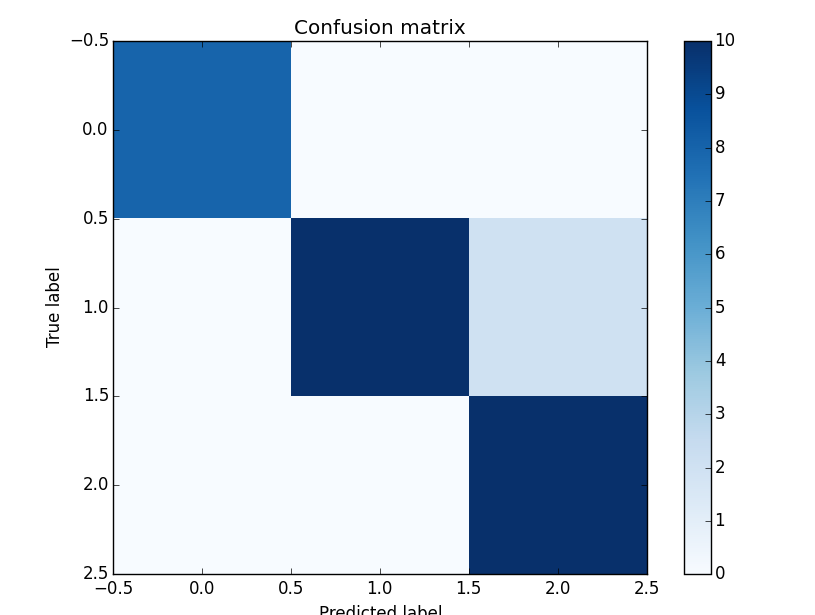
\includegraphics[scale=.5]{svm_cm_iris}
	\caption{Confusion matrix of a SVM with $C=100$, $gamma=.01$ and $rbf$ kernel when predicting samples from the Iris flower data set.}
	\label{fig:cmsvmiris}
\end{figure}

\section{Linear Dimensionality Reduction}

As presented in the previous sections, data sets with many features may present a series of issues: difficult visualization, high performance requirements, noise etc. In this section, it will be discussed methods related with linear dimensionality reduction, i.e., the shrinking of data sets by transformation and/or removal of features, while minimizing information loss.

Consider the data set $K$. $K$ has its samples expressed by two similarly scaled dimensions. It is clear, however, that the samples follow a very particular distribution:

\begin{figure}[H]
    \centering
	\captionsetup{justification=centering}

	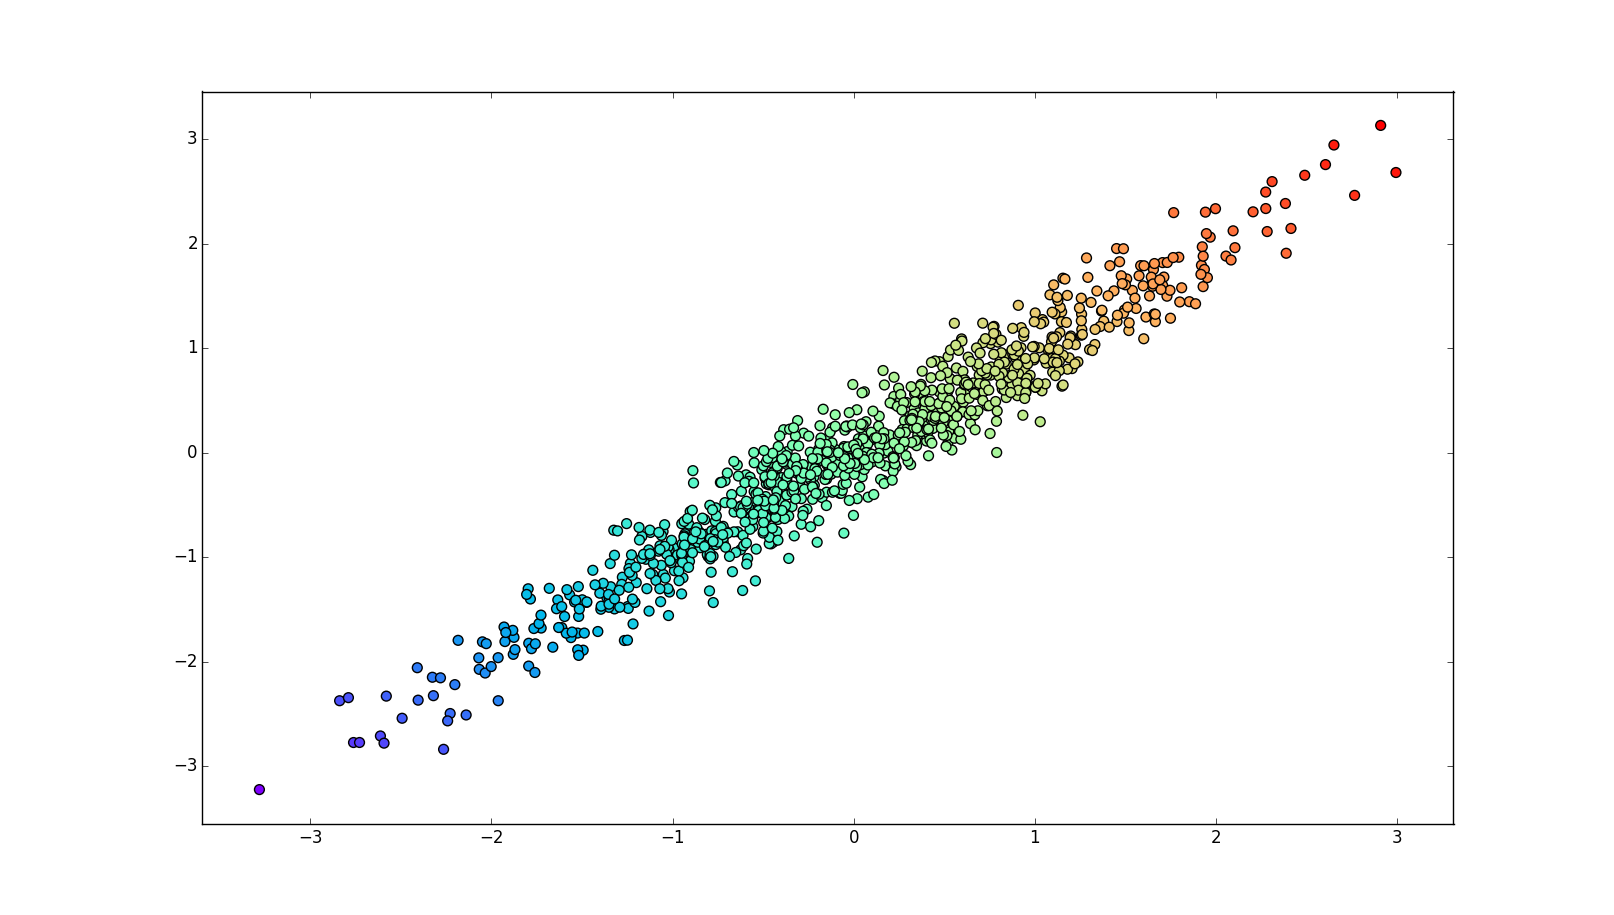
\includegraphics[width=.8\linewidth]{datasetr}
	\caption{The data set $K \in \mathbb{R}^2$.}
	\label{fig:datasetr}
\end{figure}

Additionally, something interesting can be observed when analyzing the covariance matrix of $K$: as it is not a diagonal matrix, the variance of $x$ from its mean somehow correlates with the variance of $y$. \cite{pcajon2003}

\begin{table}[H]
	\centering
	\begin{tabular}{|c|c|c|}
		\hline
			& \textbf{x} & \textbf{y} \\\hline
		\textbf{x} & 1.26682132  & 1.29158697 \\\hline
		\textbf{y} & 1.29158697  & 1.40358478 \\\hline
	\end{tabular}
	\caption{Covariance between the components of $K$.}
\end{table}

\subsection{Principal Component Analysis}

As in $K$, some data sets follow certain distributions that are majorly contained in a few orthogonal components, where a component is the result of a linear combination of the original features.

Principal Component Analysis (PCA) is a statistical technique that attempts to transform a $n$-dimensional data set $X$ into a $m$-dimensional data set $Y$, where, hopefully, $k \ll n$. Furthermore, the dimensions of $Y$ will necessarily be orthogonal components aligned with the direction in which the variance of samples in $X$ is maximum, commonly referred to as \textbf{principal components}. \cite{pca1989} In figure \ref{fig:datasetrpc}, the orange and purple vectors are the principal components of the data set $K$.

\begin{figure}[H]
	\centering
	\captionsetup{justification=centering}
	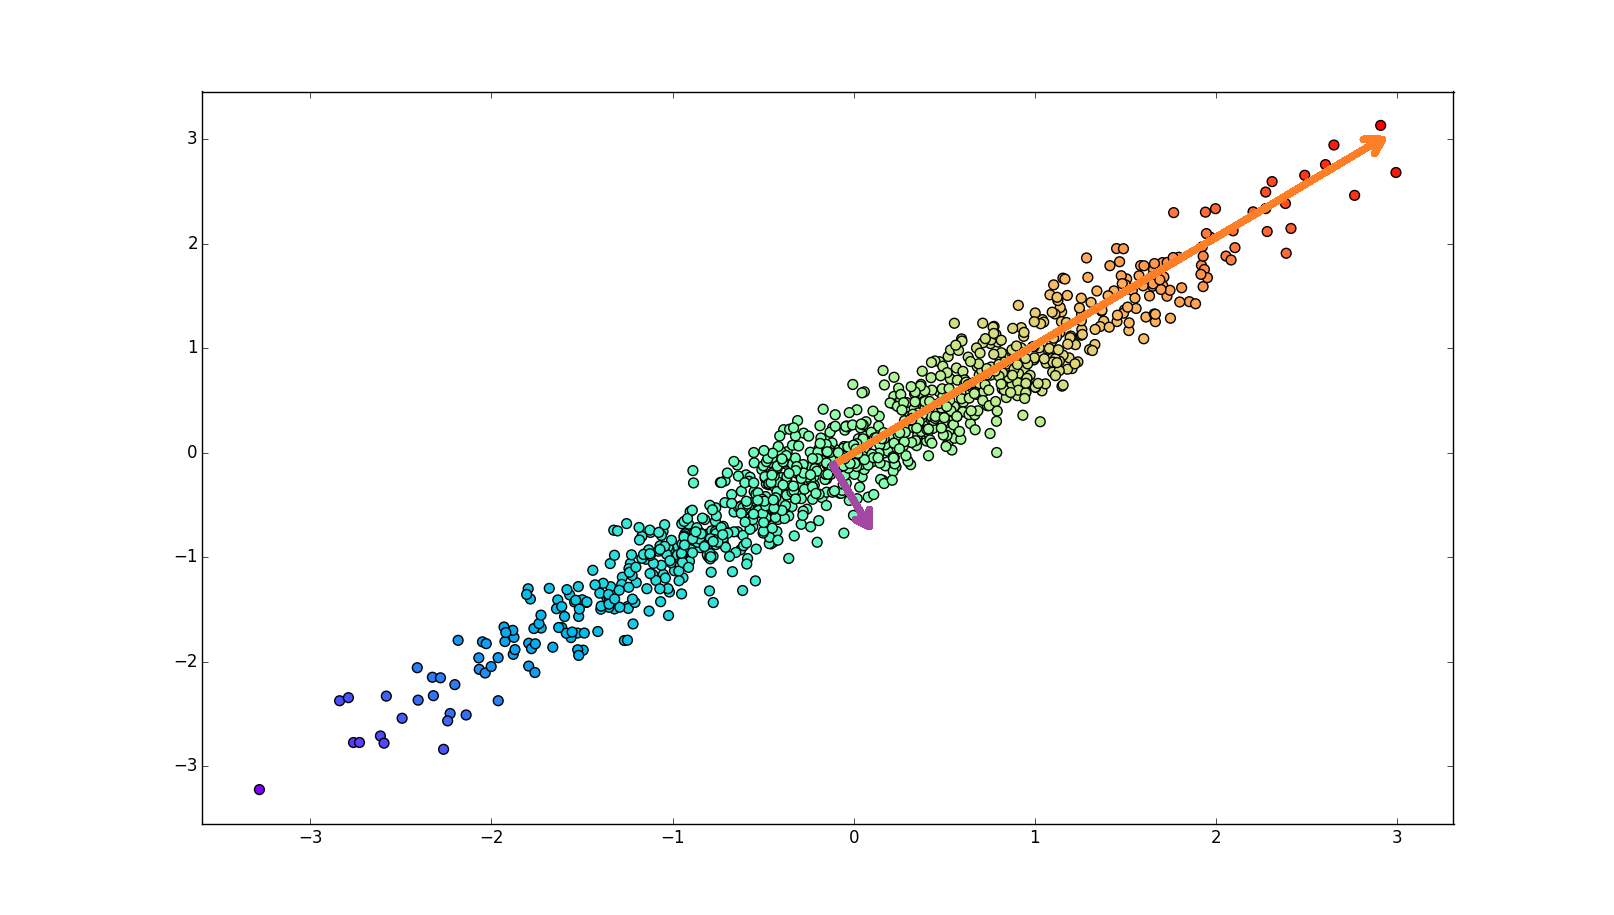
\includegraphics[width=.8\linewidth]{datasetrpc}
	\caption{The principal components of $K$.}
	\label{fig:datasetrpc}
\end{figure}

\subsubsection{Study of the PCA Algorithm}

Let $D$ be a dataset with $n$ samples and $f$ features and $X=HD$, where $H$ is the centering matrix. Our goal is to find which are the principal components of the covariance matrix $\Sigma_X$.
\begin{align}
	\label{eq:pca-cov}
	\Sigma_X=\frac{1}{n} X^TX
\end{align}

Using the \textbf{Singular Value Decomposition} method described in section \ref{sec:svd}, we known that
\begin{align}
	\label{eq:pca-svd}
	X = U\Sigma V^T
\end{align}

Needless to say, $\Sigma$ is the diagonal matrix of singular values, not to be mistaken by the covariance matrix $\Sigma_X$.

From \ref{eq:pca-cov} and \ref{eq:pca-svd}:
\begin{align*}
	\Sigma_X &= \frac{1}{n} X^TX \\
	&= \frac{1}{n} (U\Sigma V^T)^TU\Sigma V^T \\
	&= \frac{1}{n} V\Sigma^2 V^T
\end{align*}

Which entails that $V$ is the orthonormal matrix with $\Sigma_X$'s eigenvectors as columns, whereas $\Sigma$ contains the correspondent eigenvalues $\sigma_{ii}^2$ associated with $v_i\in V$. $v_i\in V$ is, in fact, a principal component of $X$ and its associated eigenvalue $\sigma_i$ module gives $X$ spectral radius. As we are interested in the dimensions that give most variance, keep only the $m\in\mathbb{R}$ most significant eigenvalues and their correspondent eigenvectors.

Finally, it also worth remarking once again that the principal components are linear combinations of the original features (the canonical base) and $V$ is the change-of-basis matrix from the generated base to the canonical. Naturally, $V^{-1}$ is a change-of-basis matrix from the original space to the one that is generated by the principal components. Formally, if $x$ is a sample (row vector) from the $X$ data set, its project $y$ is defined as:

\begin{align*}
	Vy^T &= x^T \\
	y^T  &= V^{-1}x^T
\end{align*}

In the other hand, $V$ is orthogonal, hence $V^{-1}$ exists and it is equal to $V^T$: \begin{align*}
	y^T &= V^Tx^T \\
	y &= (V^Tx^T)^T \\
      &= xV
\end{align*}

\subsubsection{Formalization of the PCA Algorithm}

Let $D$ be a data set with $n$ samples and $f$ features and $m\in\mathbb{R}$ the number of dimensions desired for the reduced data set. \cite{pca2002} \cite{pcapy}

\begin{enumerate}
	\item Find $X=HD$, where $H$ is the centering matrix.

	\item Calculate the covariance matrix $\Sigma_X$.

	\item Use singular value decomposition to find the eigenvalues $\lambda = \{\lambda_i\}$ and eigenvectors $V = \{v_i\}$ of $\Sigma_X$.

	\item Sort the eigenvalues by their absolute value in descending order and select the first $m$ ones and their respective eigenvectors.
\end{enumerate}

\subsubsection{Extensions: Kernel PCA}

Firsly, Kernel PCA is out of this project's scope. The method will be briefly mentioned, though, as it will later compared to Isomap.

\subsection{Multidimensional Scaling}

Alternatively to PCA, Multidimensional Scaling (or simply MDS) can be used to reduce the dimensionality of a data set. The method has, however, an extensive application domain and often appears in the literature in different contexts. An example of this is the problem of, given a set of objects $O$ and a dissimilarity measurement $\delta_{rs}, \forall (r, s) \in O\times O$, finding a suitable representation in the $\mathbb{R}^n$ for the objects in $O$. \cite{cox2001}

For this project, we study the \textbf{classic MDS}. That is, when the dissimilarities considered are the euclidean distances between coordinates in the $\mathbb{R}^n$.

\subsubsection{Study of the MDS}

If $\delta = [\delta_{rs}]_{n\times n}$ is the dissimilarity matrix, where $\delta_{rs}$ represents the euclidean distances between two samples $x_r, x_s\in \mathbb{R}^m$ from the data set $[X]_{n\times m}$ induced by the $L2$-norm. In other words,
\begin{align}
\label{eq:basemds}
\begin{split}
  \delta_{rs}  &= \sqrt{\sum_i (x_{ri}-x_{si})^2} \\
  &\iff \\
  \delta_{rs}^2 &= \sum_i (x_{ri}-x_{si}^2) \\
  &= (x_r-x_s)\cdot (x_r-x_s) \\
  &= x_r\cdot x_r + x_s\cdot x_s -2x_r\cdot x_s
\end{split}
\end{align}

Now consider the inner product matrix $B=XX^T$, where $b_{rs}=x_{.r}\cdot x_{.s}$. Given that $B$ can be decomposed as $U\Sigma U^T=U\Sigma^\frac{1}{2} \Sigma^\frac{1}{2} U^T=U\Sigma^\frac{1}{2} (U\Sigma^\frac{1}{2})^T = XX^T\iff X=U\Sigma^\frac{1}{2}$, if we can derive $B$ from \ref{eq:basemds}, it will be possible to apply the same decomposition considered in PCA to find a new data set $Y$ which is a reduction of $X$. \cite{cox2001}

Firstly, we will assume that $Y$ is centered in the origin (i.e., $Y$ has its features' means equal to zero):
\begin{align}
\sigma_f = \sum_i y_{if} = 0, \forall f\in [0, m)
\end{align}

Now, \ref{eq:basemds} $\implies$
\begin{align}
\label{eq:xsderivation}
\begin{split}
\frac{1}{n} \sum_r \delta_{rs}^2
&= \frac{1}{n} \sum_r (x_r\cdot x_r + x_s\cdot x_s -2x_r\cdot x_s) \\
&= \frac{1}{n} \sum_r x_r\cdot x_r + \sum_r x_s\cdot x_s -2 \sum_r x_r\cdot x_s \\
&= \frac{1}{n} \sum_r x_r\cdot x_r + nx_s\cdot x_s -2 \sum_r 0\cdot x_s \\
&= \frac{1}{n} \sum_r x_r\cdot x_r + x_s\cdot x_s \\
&\iff \\
x_s\cdot x_s &= \frac{1}{n} (\sum_r \delta_{rs}^2 - \sum_r x_r\cdot x_r)
\end{split}
\end{align}

Similarly to \ref{eq:xsderivation},
\begin{align}
\label{eq:xrderivation}
\begin{split}
x_r\cdot x_r &= \frac{1}{n} (\sum_s \delta_{rs}^2 - \sum_s x_s\cdot x_s)
\end{split}
\end{align}

Putting \ref{eq:xsderivation} and \ref{eq:xrderivation} back in \ref{eq:basemds}:
\begin{align}
\label{eq:xrsderivation}
\begin{split}
\delta_{rs}^2 &= \frac{1}{n} (\sum_s \delta_{rs}^2 - \sum_s x_s\cdot x_s + \sum_r \delta_{rs}^2 - \sum_r x_r\cdot x_r) -2x_r\cdot x_s \\
&\implies \\
x_r\cdot x_s &= -\frac{1}{2} (\delta_{rs}^2 - \frac{1}{n} [\sum_s \delta_{rs}^2 - \sum_s x_s\cdot x_s + \sum_r \delta_{rs}^2 - \sum_r x_r\cdot x_r])\\
&= -\frac{1}{2} (\delta_{rs}^2 - \frac{1}{n} [\sum_s \delta_{rs}^2 + \sum_r \delta_{rs}^2 - 2\sum_r x_r\cdot x_r])\\
\end{split}
\end{align}

To eliminate the $x_r\cdot x_r$ term from \ref{eq:xrsderivation}:
\begin{align}
\label{eq:msd-xrr}
\begin{split}
\frac{1}{n^2} \sum_s\sum_r\delta_{rs}^2 &= \frac{1}{n^2} \sum_s\sum_r(x_r\cdot x_r + x_s\cdot x_s -2x_r\cdot x_s)\\
&= \frac{1}{n^2}\sum_s(\sum_r x_r\cdot x_r + \sum_r x_s\cdot x_s -2\sum_r x_r\cdot x_s)\\
&= \frac{1}{n^2}\sum_s(\sum_r x_r\cdot x_r + n x_s\cdot x_s) \\
&= \frac{1}{n^2}(n \sum_r x_r\cdot x_r + n \sum_s x_s \cdot x_s) \\
&= \frac{1}{n^2} 2n \sum_r x_r\cdot x_r \\
&= \frac{2}{n} \sum_r x_r\cdot x_r
\end{split}
\end{align}

Finally, applying \ref{eq:msd-xrr} on \ref{eq:xsderivation}:
\begin{align}
\label{eq:mds-defb}
\begin{split}
B_{rs} = x_r\cdot x_s = -\frac{1}{2} (\delta_{rs}^2 - \frac{1}{n} [\sum_s \delta_{rs}^2 + \sum_r \delta_{rs}^2 - \frac{1}{n}\sum_s \sum_r \delta_{rs}^2])
\end{split}
\end{align}

From \ref{eq:mds-defb}, it becomes clear that $B$ is, in fact, the double centering of the matrix $A=-\frac{1}{2}\delta^2$. I.e., $B=HAH$. Spectral decomposition can now be performed onto $B$, resulting in the matrices $\Sigma$ and $U$.

Finally, we can sort the eigenvalues (and their respective eigenvectors, the columns of $U$) in decrease order and keep only the ones that offer greater variance.

\begin{remark}
	As euclidean distances were used to build the dissimilarity matrix $\delta$, $B$ is indubitably positive semidefinite, hence $\Sigma_i \ge 0, \forall i\in [0, n)$. However, negative eigenvalues might appear if other dissimilarity measurement were to be used. In these cases, one might consider to simply ignore such components.
\end{remark}

\subsubsection{Formalization of the Multidimensional Scaling Method}

Let $X$ be a data set with $n$ samples and $f$ features and $m\in\mathbb{R}$ the number of dimensions desired for the reduced data set. \cite{cox2001}

\begin{enumerate}
	\item Calculate the dissimilarity matrix $[\delta]_{rs}$, where $\delta_{rs} = \sqrt{\sum_i (x_{ri} - x_{si})^2}$
	\item Calculate the matrix $A=-\frac{1}{2}\delta_{rs}^2$ and $B=HAH$, where $H$ is the centering matrix.

	\item Use spectral decomposition to find the matrices $\Sigma$ and $U$.

	\item Select the $m$ greatest eigenvalues in $\Sigma$. From these, create the matrices $\Sigma'=[\sigma'_{m\times m}]$ and $U'=[u'_{n\times m}]$, where each column $i$ contains the eigenvector associated with $\sigma'_i$.

	\item Construct the $m$-dimensional embedding $Y=U'\Sigma'$
\end{enumerate}

\subsection{Evaluating Reductions}

``Often it is the researcher's past experience with MDS and his or her judgment that
ultimately determine whether the fit of a particular MDS solution is acceptable or not." \cite{naes1996multivariate}

Although the factors that determine what is a ``good" reduction are strongly influenced by particularities of the problem in hand, some measures were developed to attempt to somehow formalize it. One in particular, which recurrently appears in literature, is known as the \textbf{Kruskal's stress}.

Intuitively, Kruskal's stress \cite{naes1996multivariate} considers reductions that preserve dissimilarities between samples a better fit that the ones which highly distort them. Formally, let $X_{n \times f}$ be a data set with $n$ samples and $f$ dimensions, $Y_{n \times p}$ its reduction to $p$ dimensions, and the dissimilarity measurements $\delta_{ij}$ and $\hat{\delta}_{ij}$ defined for all samples $i$ and $j$ in $X$ and $Y$, respectively:
\begin{align*}
	Stress &= [\frac{\sum_i \sum_j (\delta_{ij} - \hat{\delta}_{ij})^2}{\sum_i \sum_j \delta_{ij}^2}]^{\frac{1}{2}}
\end{align*}

From the formula above, {\em Stress} is visibly contained in the interval $[0, 1]$, where 0 represents the best possible fit (all dissimilarities are the same), while 1 represents the worse.

\subsection{Classification and Regression Over Linearly Reduced Data Sets}
\label{sec:experiments_linear_ds}

This section reports the performance of classifiers and regressors over determined data sets and their reduced forms. All experiments followed the format bellow:

\begin{enumerate}
	\item The data set $X_{n \times m}$ was loaded.
	\item Grid Search was executed over the original data set.
	\item for $d \in D \subset \mathbb{N} \mid d \in D \implies d < m$:
	\begin{enumerate}
		\item The $d$-dimensional embedding $Y$ of $X$ was calculated.
		\item Grid Search was executed over $Y$.
	\end{enumerate}
\end{enumerate}

\subsubsection{$K$ Data Set}

The figure bellow illustrates the results of PCA algorithm application over the artificial $K$ data set. Notice that, for the second application, it correctly chose to discard the vertical dimension, as the samples offer less variability in this component.

\begin{figure}[H]
	\centering
	\captionsetup{justification=centering}

	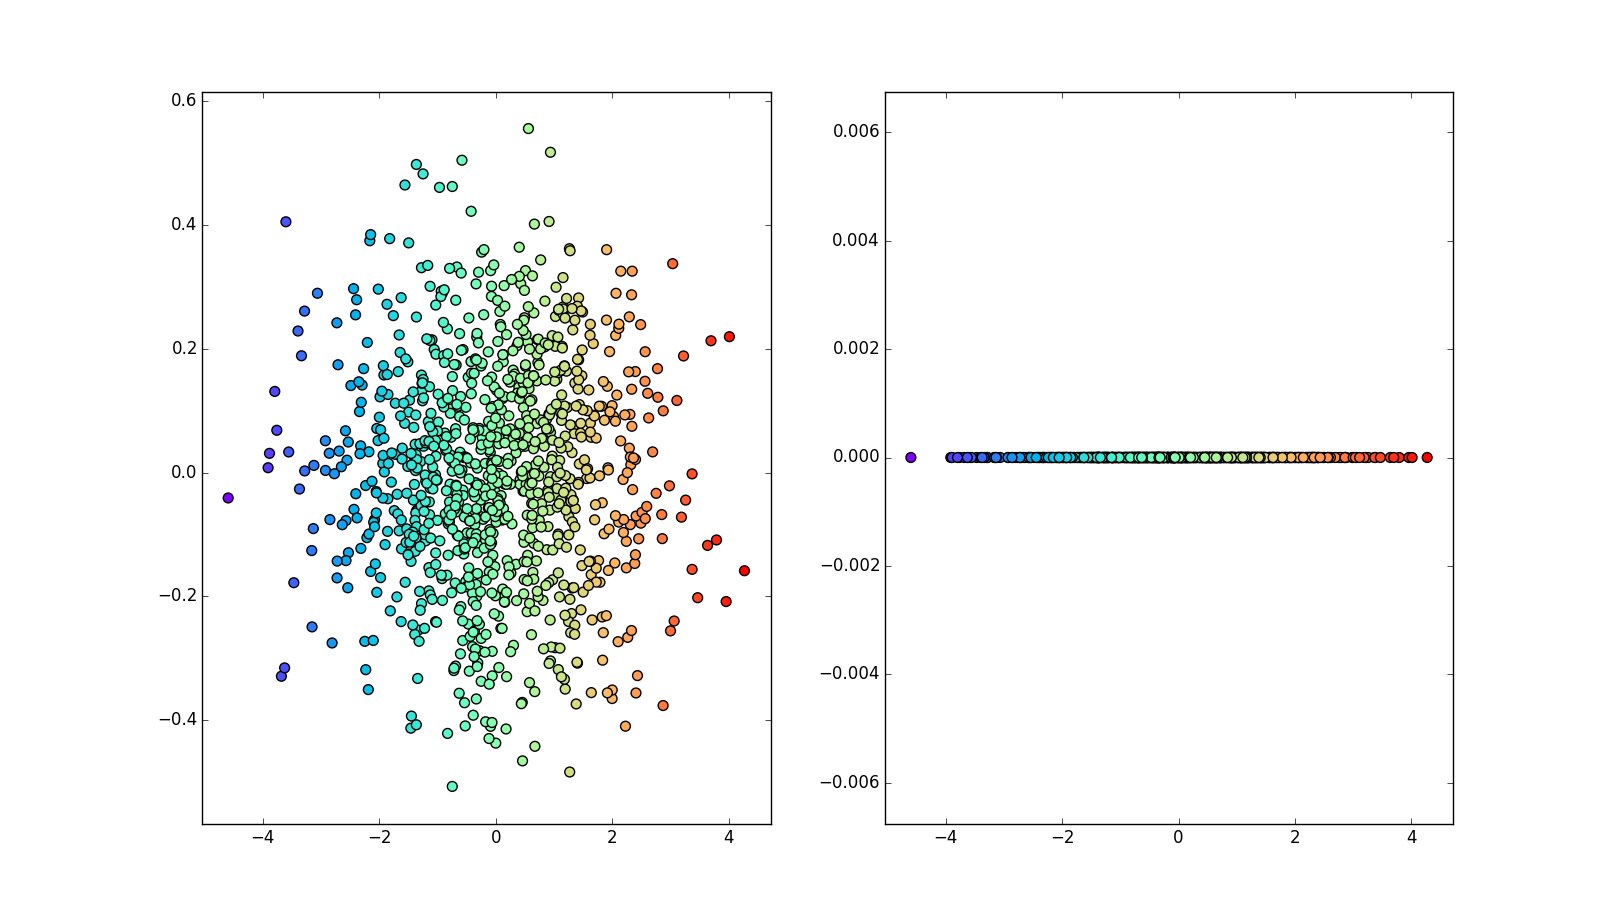
\includegraphics[width=.9\linewidth]{datasetrpca}
	\caption{The PCA algorithm reducing $K$ to 2 and 1 dimension, respectively.}
	\label{fig:datasetrpca}
\end{figure}

\begin{table}[H]
	\centering
	\begin{tabular}{|c|c|c|c|}
		\hline
		& \textbf{Original data} & \textbf{Reduced data ($\mathbb{R}^2$)} & \textbf{Reduced data ($\mathbb{R}$)} \\\hline
		\textbf{Pred. accuracy} & .98 & .98 & .99 \\\hline
		\textbf{GridSearch time} & 1.15 s & .84 s & 1.26 s \\\hline
		\textbf{Reduction time} & - & 0.995 ms & 1.118 ms \\\hline
		\textbf{Stress} & - & 0 & .0399 \\\hline
		\textbf{Data size} & 15.62 KB & 15.62 KB & 7.81 KB \\\hline
	\end{tabular}

	\caption{Description of predictions and reduction performance for $K$.}
\end{table}

From the table above, one can also observe how Kruskal's stress might not be an appropriate quality measurement, given a specific domain. Indeed, for data set $K$, stress increase resulted from the removal of one of the components did not imply on prediction accuracy decrease.

\subsubsection{The Iris Flower Data Set}

The Iris flower being reduced from 4 to 2 features. Although the data set became non-linearly separable, classes are still somewhat organized in different clusters.

\begin{figure}[H]
	\centering
	\captionsetup{justification=centering}

	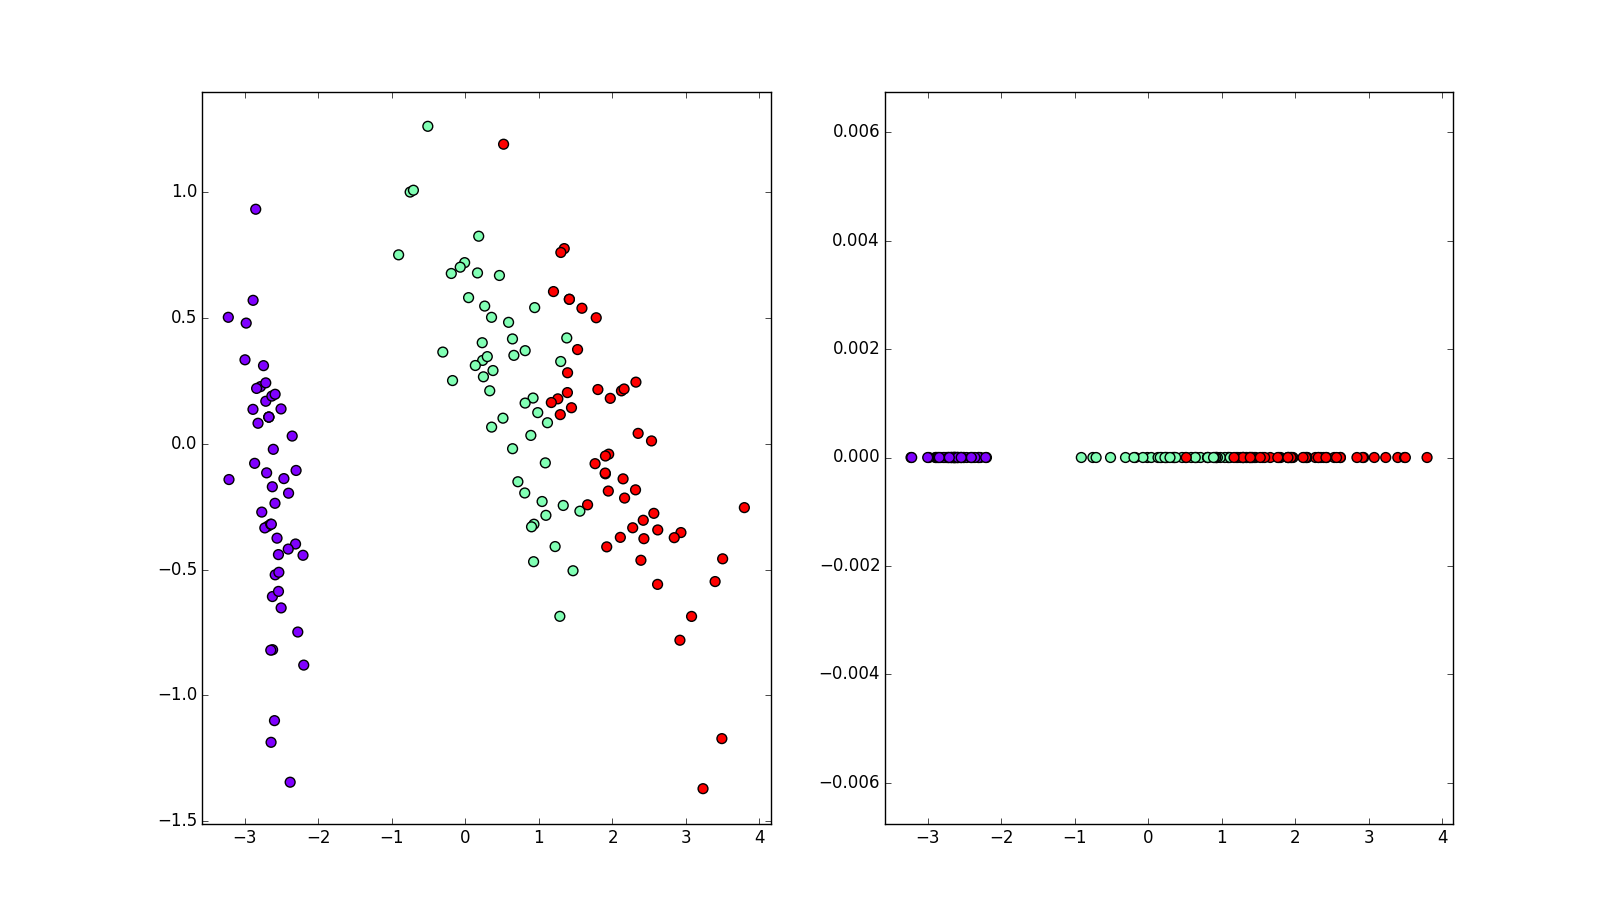
\includegraphics[width=\linewidth]{dsirispca}
	\caption{The PCA algorithm reducing the Iris flower to 2 and 1 dimension, respectively.}
	\label{fig:dsirispca}
\end{figure}

\begin{table}[H]
	\centering

	\begin{tabular}{|c|c|c|c|}
		\hline
		& \textbf{Original data} & \textbf{Reduced data ($\mathbb{R}^2$)} & \textbf{Reduced data ($\mathbb{R}$)} \\\hline
		\textbf{Pred. accuracy} & .99 & .97 & .94 \\\hline
		\textbf{GridSearch time} & 1.71 s & 1.64 s & 1.78 s \\\hline
		\textbf{Reduction time} & - & 0.995 ms & 1.118 ms \\\hline
		\textbf{Stress} & - & .0418 & .1095 \\\hline
		\textbf{Data size} & 4.68 KB & 2.34 KB & 1.17 KB \\\hline
	\end{tabular}

	\caption{Description of predictions and reduction performance for Iris flower.}
\end{table}

\subsubsection{The Digits Data Set}

Digits data set is composed by 1797 samples, 64 features and 10 classes. Each sample is a 8x8 image of a hand-written digit from 0 to 9.

\begin{figure}[H]
	\centering
	\captionsetup{justification=centering}
	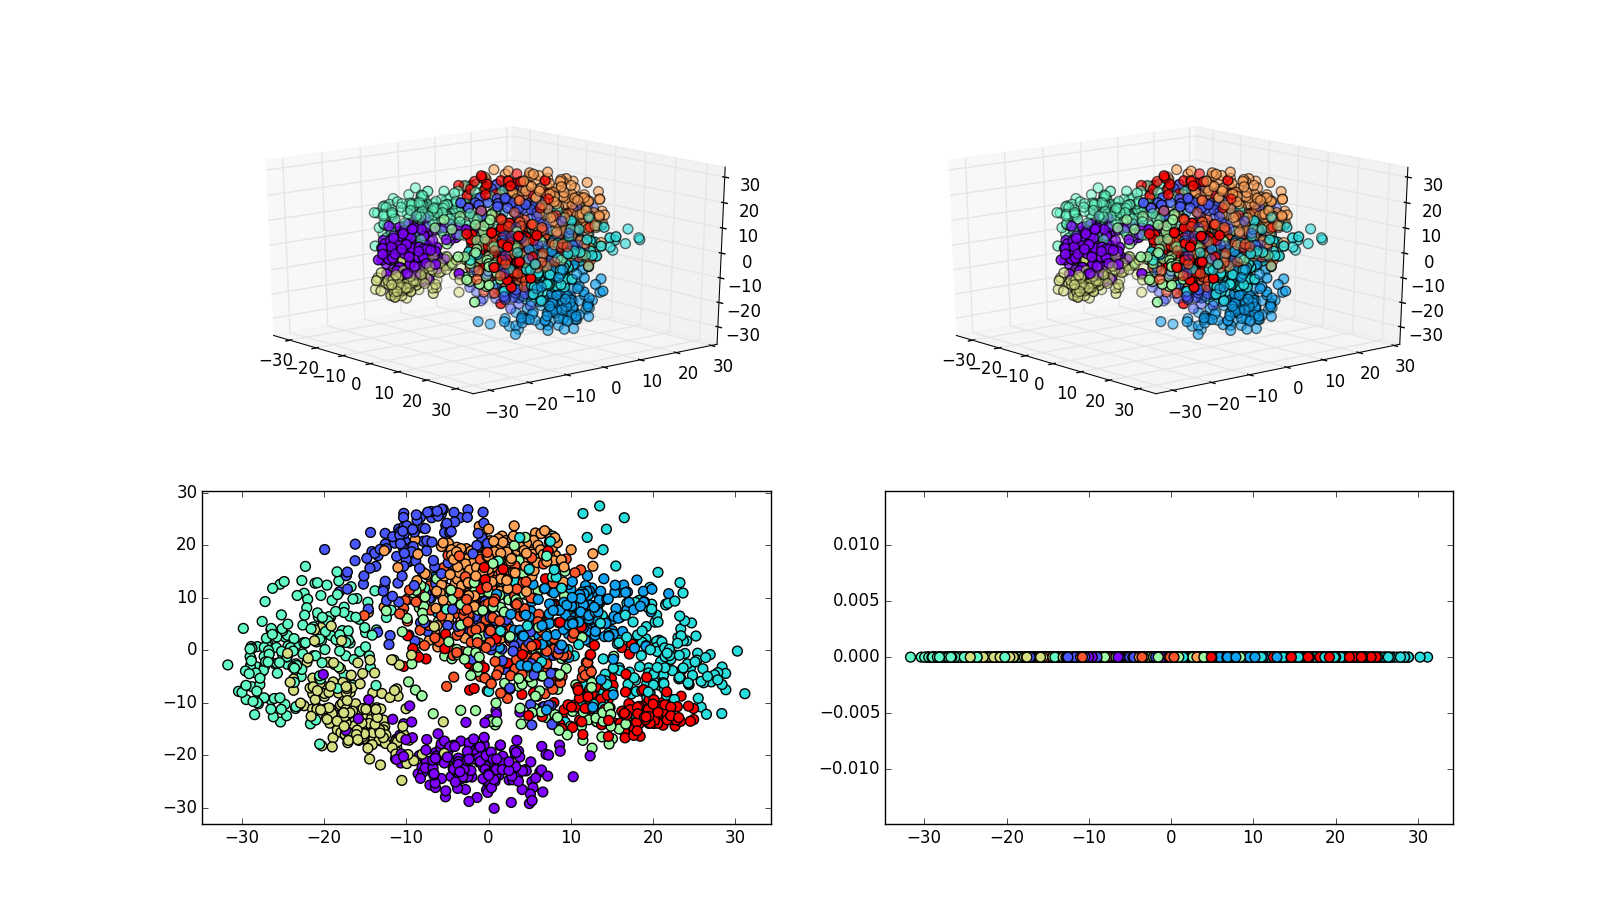
\includegraphics[width=\linewidth]{dsdigitspca}
	\caption{Digits data set reduced to 10, 3, 2 and 1 dimension, respectively.}
	\label{fig:dsdigitspca}
\end{figure}

\begin{table}[H]
	\centering
	\begin{tabular}{|c|c|c|c|c|c|}
		\hline
		& \textbf{$\mathbb{R}^{64}$} & \textbf{$\mathbb{R}^{10}$} & \textbf{$\mathbb{R}^3$} & \textbf{$\mathbb{R}^2$} & \textbf{$\mathbb{R}$} \\\hline
		\textbf{Pred. accuracy}   & .98 & .95 & .74 & .64 & .39 \\\hline
		\textbf{GridSearch time} & 8.51 s & 21.33 s & 151.04 s & 132.18 s & 113.78 s \\\hline
		\textbf{Reduction time} & - & 0.02 s & 0.01 s & 0.01 s & 0.01 s \\\hline
		\textbf{Stress} & - & .1594 & .4218 & .5405 & .7092 \\\hline
		\textbf{Data size} & 898.5 KB & 140.39 KB & 42.11 KB & 28.07 KB & 14.03 KB \\\hline
	\end{tabular}

	\caption{Description of predictions and reduction performance for Digits.}
\end{table}

Notice that it was possible to eliminate 54 dimensions, consistently reducing the data set size, and only suffering 3\% of prediction accuracy loss. The score drastically decreased, however, when more dimensions were removed. Furthermore, accuracy decrease was followed by stress increase.

\newpage
\section{Nonlinear Dimensionality Reduction}

Although PCA has presented promising results in the previous section, hence its great popularity in dimensionality reduction problems, there are many examples in which PCA will fail in its task. Consider the example bellow:

\begin{figure}[H]
	\centering
	\captionsetup{justification=centering}

	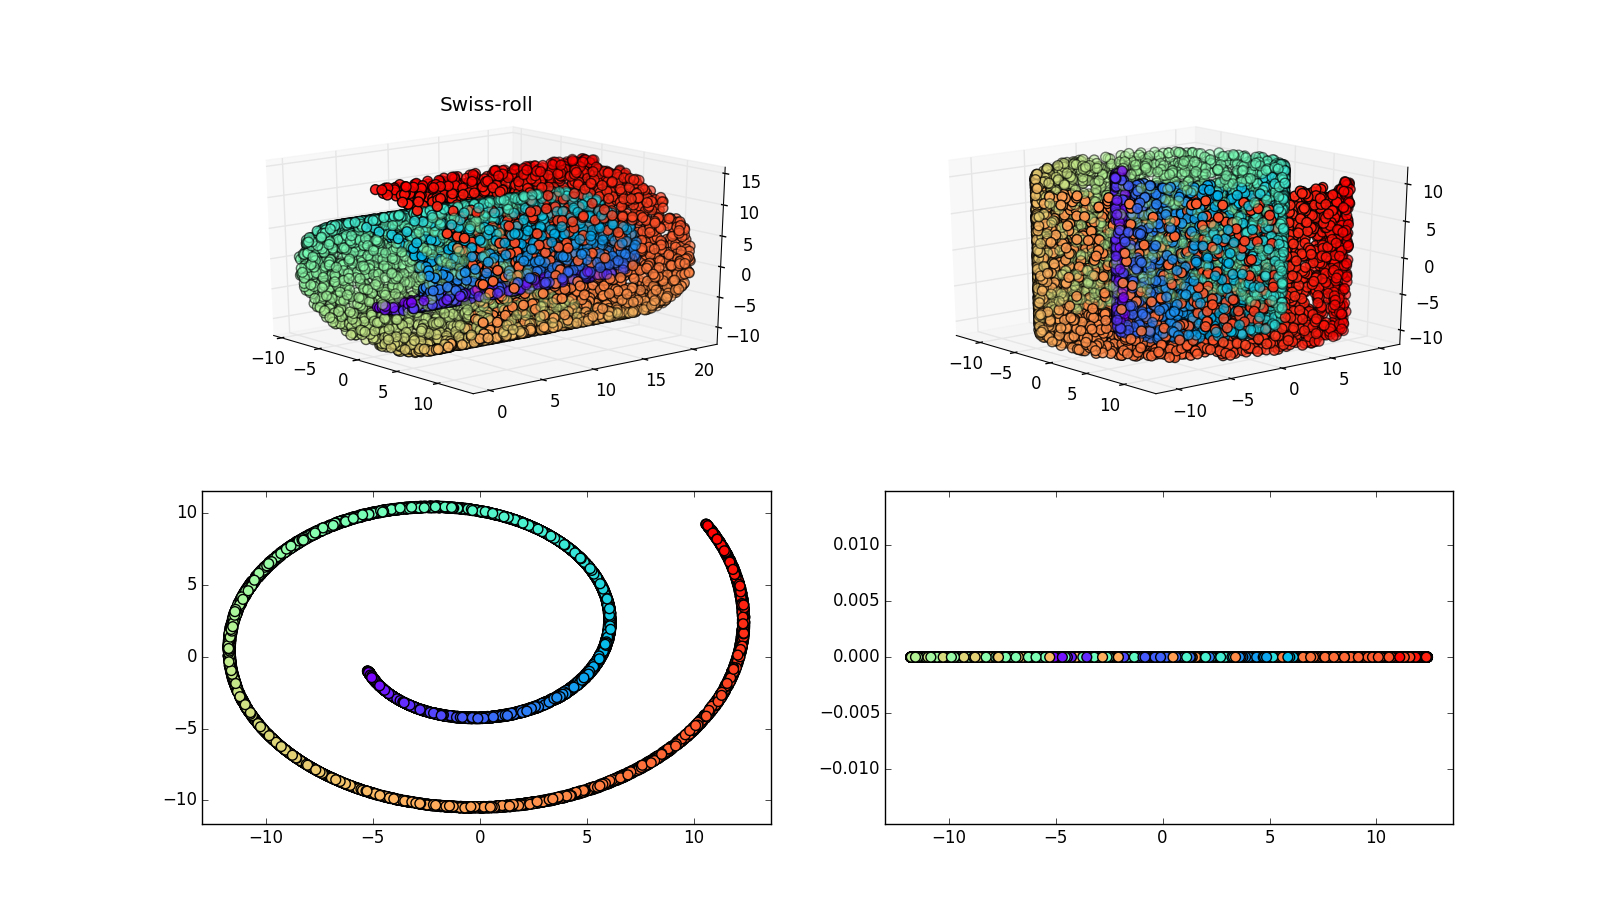
\includegraphics[width=\linewidth]{swiss_pca}
	\caption{The \textbf{Swiss-roll manifold} and its reductions to 3, 2 and 1 dimensions, respectively, using the PCA algorithm.}
	\label{fig:swiss_pca}
\end{figure}

Looking at figure \ref{fig:swiss_pca} (specially in the last reduction, to a single dimension), it becomes clear that PCA has a big draw back: it assumes that the data lies on a liner subspace \cite{cay2005} and, therefore, applying linear transformations to it will rotate and scale it, without distort the original data structure. When this assumption does not hold, PCA will incorrectly extract the underlying structure, possibly mixing very dissimilar samples.

The table bellow describes a regression attempt over the data sets illustrated in figure \ref{fig:swiss_pca}, were the feature being predicted is the contiguous value represented by the vertexes' colors:

\begin{table}[H]
	\centering
	\begin{tabular}{|c|c|c|c|c|}
		\hline
		& \textbf{Original data} & \textbf{Reduc. ($\mathbb{R}^3$)} & \textbf{Reduc. ($\mathbb{R}^2$)} & \textbf{Reduc. ($\mathbb{R}^1$)} \\\hline
		\textbf{Accuracy} & 1. & 1. & .68 & .54 \\\hline
		\textbf{GS time}  & 10.98 s & 10.48 s & 5.20 s & 2.59 s \\\hline
		\textbf{Reduc. time} & - & 0.038 s & 0.038 s & 0.035 s \\\hline
		\textbf{Stress} & - & 0 & .2788 & .5271 \\\hline		
		\textbf{Data size} & 23.44 KB & 23.44 KB & 15.62 KB  & 7.81 KB \\\hline
	\end{tabular}

	\captionsetup{justification=centering}
	\caption{Regression accuracy and reduction performance for the Swiss-roll data set.}
\end{table}

Clearly, linear dimensionality reduction techniques are not adequate to reduce the Swiss-roll. In fact, it is not adequate to reduce any data set lying on a nonlinear manifold.

\subsection{The Isomap Algorithm}

Firstly suggested by Tenenbaum, de Silva and Langfor, \textbf{Isometric Mapping} (or Isomap) assumes that the data lies near a smooth manifold. If the assumption is reasonable, it is be possible to explore concepts such as neighborhood and local linearity to map the manifold to a linear structure before reducing it with a linear algorithm.

In this section we will discuss the Isomap algorithm and its inner workings. We will then proceed to formalize it. Finally, empirical tests results achieved during the project will be shown.

\subsubsection{Study of the Isomap Algorithm}

As the original data set might be folded, twisted or curved, \cite{ten2000} we must first find a suitable linear representation for it.

Let $S$ be our original data set, as illustrated in figure \ref{fig:mani_s}.

\begin{figure}[H]
	\centering
	\captionsetup{justification=centering}
	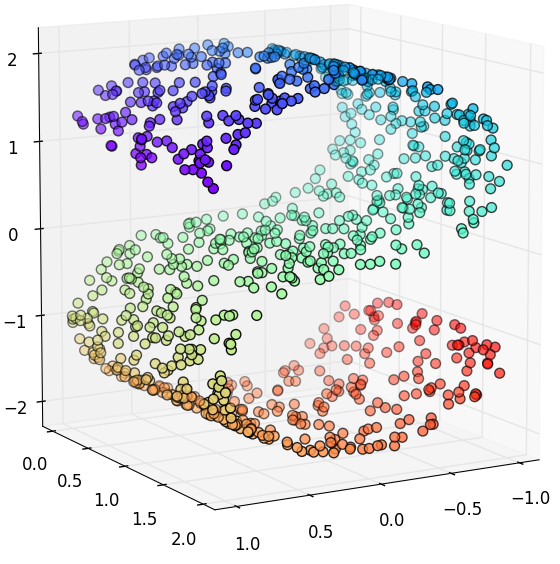
\includegraphics[width=.5\linewidth]{mani_s}
	\caption{The data set $S$, consisting of $1000$ samples and $3$ features.}
	\label{fig:mani_s}
\end{figure}

Additionally, consider the symmetric undirected weighted graph $G=(V, E)$ and $w \colon E \to \mathbb{R} \mid w(x, y) = \delta_{xy}$, where $\delta_{xy}$ is the euclidean distance between the samples $x$ and $y$ in $S$. That is,
$$\delta_{xy} = \sqrt{\sum_{i} (x_i - y_i)^2}, \forall (x, y) \in S\times S \mid x\ne y$$

Now that only distances were kept, an infinite number of n-dimensional embeddings can be found with \textbf{MDS}, as every solution can be transposed, rotated or reflected. This does not fix the non-linearity of the data, though, as the original distances strictly constraint the samples to their original pattern. In order to achieve this, \textbf{Nearest neighbor search} can be performed over $G$, resulting in the graph $H$. Nearest-neighbor search will preserve edges connecting closer samples, hence preserving local (linear) distances, but erase edges connecting samples which are far from each other (non necessarily linear). Obviously, the search parameters ($K$ or $\epsilon$) must be carefully chosen to limit the connectivity of the vertices to a small (linear) neighborhood while maintaining the graph completely connected. Ideally, $H$ will be a \textbf{mesh graph}.

\begin{figure}[H]
	\centering
	\captionsetup{justification=centering}
	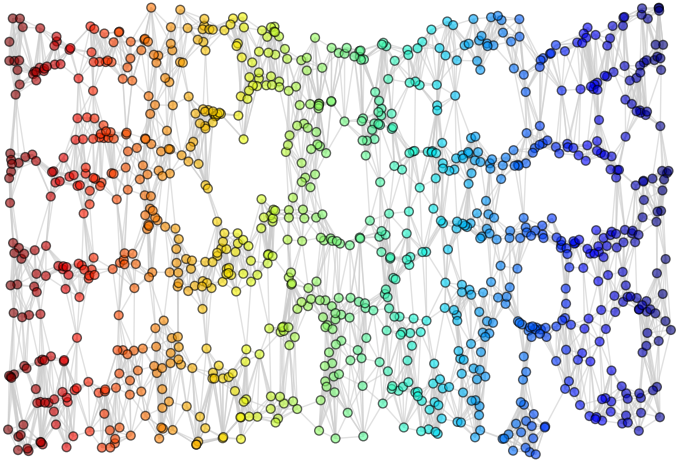
\includegraphics[width=.5\linewidth]{mani_s_3}
	\caption{The graph $H$.}
	\label{fig:mani_s_graph_h}
\end{figure}

At this moment, not all distances in $H$ are defined. This can be easily handled, though, by performing the \textbf{Floyd-Warshall} algorithm over $H$. Alternatively, $M$ can be achieved by performing \textbf{Dijkstra's algorithm} for all nodes and joining all shortest-path trees found.

Finally, $M$ is a euclidean graph which roughly lies on a hyperplane. Furthermore, the adjacency matrix associated to $M$ contains not the distance induced by the $L_2$ norm, but the geodesic pairwise distances. \cite{gho2006} The \textbf{MDS} method can now be used to construct a representation in sub-spaces of the $\mathbb{R}^n$. $S$, specifically, can be reduced to the $\mathbb{R}^2$ or $\mathbb{R}^1$:

\begin{figure}[H]
    \begin{subfigure}{.5\linewidth}
		\centering
		\captionsetup{justification=centering}
		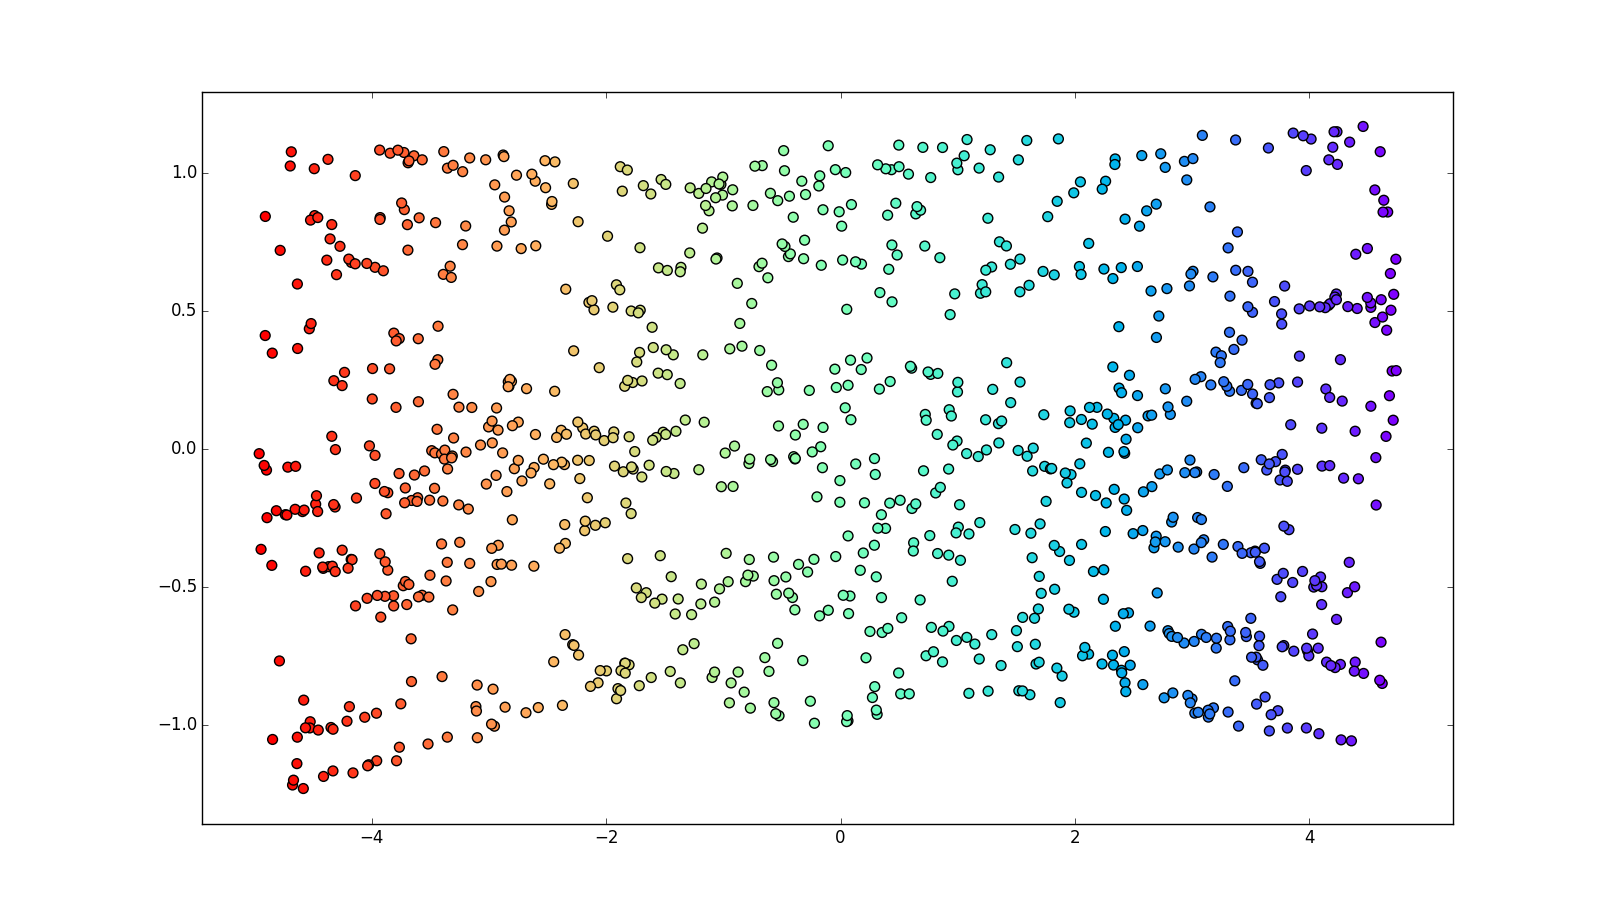
\includegraphics[width=\linewidth]{mani_s_4}
		\caption{$S$ reduced to two dimensions.}
		\label{fig:mani_s_reduced_1}
	\end{subfigure}%
	\begin{subfigure}{.5\linewidth}
		\centering
		\captionsetup{justification=centering}
		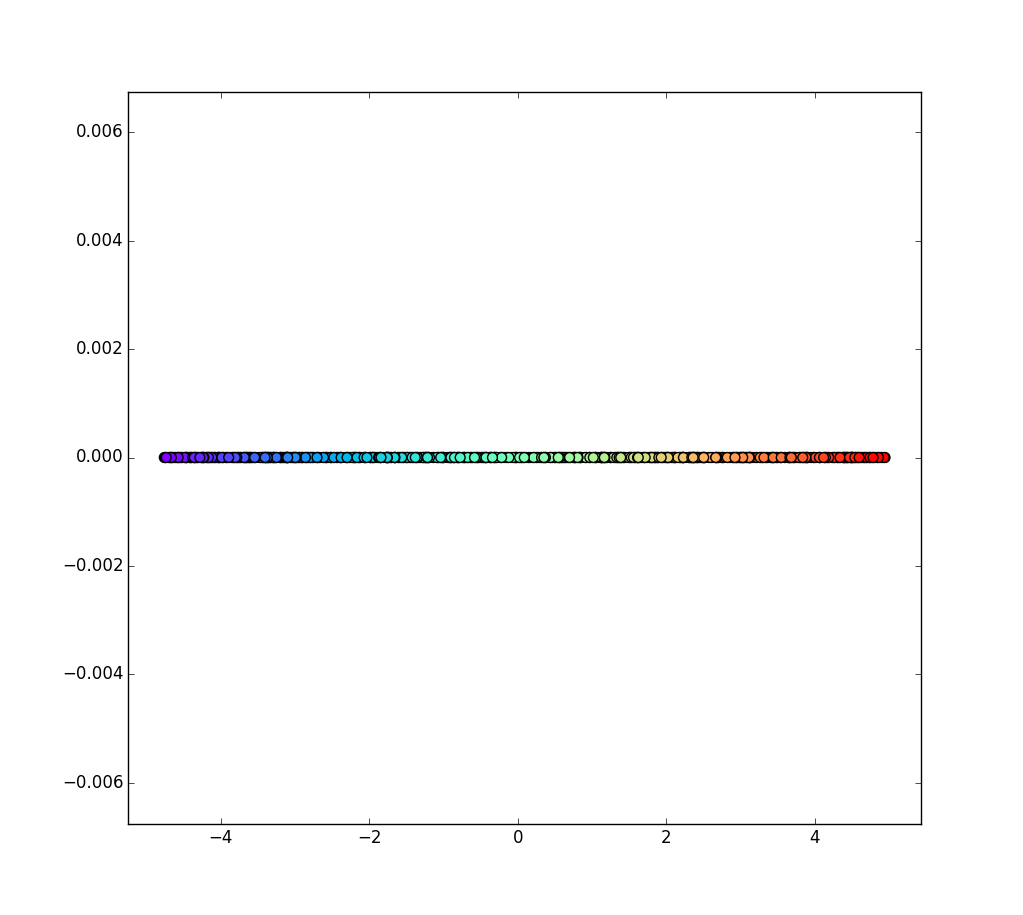
\includegraphics[width=.63\linewidth]{mani_s_5}
		\caption{$S$ reduced to one dimension.}
		\label{fig:mani_s_reduced_2}
	\end{subfigure}
\end{figure}

\newpage
\subsubsection{Formalization of the Isomap Algorithm}

Let $X$ be the original data set and $p \in \mathbb{R}$ the number of dimensions desired for the reduced data set, \cite{ten2000}

\begin{enumerate}
	\item Construct the weighted graph $G$ from the distances pairwise $\delta_{xy}, \forall (x, y) \in S \times S, x \ne y$ and find the graph $H$ by applying the \textbf{nearest-neighbor algorithm} on the graph $G$.

	\item Compute the shortest path graph $M$ between all pairs of nodes from graph $H$. This might be done by the \textbf{all-pairs Dijkstra's} or by the \textbf{Floyd-Warshall} algorithm.

	\item Use $M$ to construct the $p$-dimensional embedding using the \textbf{MDS} algorithm.
\end{enumerate}

\subsubsection{Computational Complexity}
\label{sec:isocomplexity}

If $n$ is the number of training samples, $f \in \mathbb{R}$ the number of features and $k \in \mathbb{R}$ the number of nearest neighbors:

\begin{enumerate}
	\item The time complexity associated with building the neighborhood graph is $O(n^2)$, whereas the space necessary to represent the distances kept is $n^2$.
	\item Algorithms for finding shortest path graph can be executed in-place and do not increase space complexity. Regarding time complexity, however:
	\begin{enumerate}
		\item Dijkstra's algorithm implementation using Fibonacci Heaps have time complexity $O(nk + n \log n)$. As the algorithm must be calculated for each node, this step has time complexity $O[n^2(k + \log n)]$.
		\item Alternatively, using the Floyd-Warshall algorithm, this step has time complexity equals to $O(n^3)$.
	\end{enumerate}
	\item Taking $O(n^3)$ time steps to calculate the spectral decomposition, MDS clearly is the bottleneck of the entire algorithm. \cite{cay2005} \cite{silva2002global} As for space complexity, $O(f^2 + nf)$ is required for storing the matrices $\Sigma$ and $U$.
\end{enumerate}

The time complexity of the Isomap algorithm (when using Dijkstra's) is, therefore, $O[n^2 + n^2(k + \log n) + n^3]$, and the space complexity is $O(n^2 + f^2 + nf)$.

\begin{experiment}[Timing the Isomap Algorithm]
	Consider the data set \textbf{Digits} with 1797 samples and 64 features. The following table indicates the time duration for each step of the Isomap algorithm when reducing Digits to 3 dimensions:
	
	\begin{table}[H]
		\centering
		\begin{tabular}{|l|r|}
			\hline
			\textbf{Pairwise distances from data set} & .44 s \\\hline
			\textbf{K Nearest Neighbors Search} & 1.3 s \\\hline
			\textbf{All Pairs Dijkstra's} & 51.44 s\\\hline
			\textbf{MDS} & 118.84 s \\\hline
			\textbf{Total Time} & 172.69 s \\\hline
		\end{tabular}
		
		\caption{Listing of time spent on each step of the Isomap algorithm.}
	\end{table}
	
	As expected, most of the time (68.81\%) was spent executing MDS.
\end{experiment}

In practice, Isomap's time complexity of $O[n^2 + n^2(k + \log n) + n^3]$ makes it unsuitable for data sets with high number of samples. This is illustrated in Shi and Gu's experiments: Isomap could not reduce data sets with more than 6000 samples in reasonable time. \cite{shi2012fast}

\begin{experiment}
	Let \textbf{Spam} be a data set with 4601 samples and 57 features. The table bellow describes the time necessary for the implemented Isomap and sk-Isomap (the algorithm from the \href{http://scikit-learn.org}{scikit-learn} library) to reduce Spam to 3 dimensions:
	
	\begin{table}[H]
		\centering
		\begin{tabular}{|c|c|}
			\hline
			\textbf{Algorithm} & Time \\\hline
			\textbf{Isomap} & 29.9 m \\\hline
			\textbf{sk-Isomap} & 10.76 s \\\hline
		\end{tabular}
		
		\caption{Timing the implemented Isomap and scikit-learn's implementation.}
	\end{table}

	The implemented Isomap required almost 30 minutes to reduce Spam.
	Surprisingly, scikit-learn's implementation executed incredibly fast. A set of factors contribute for this result:

	\begin{itemize}
		\item \textbf{Ball Tree} is used for efficient neighbor search (requiring only $O(f n \log k \log n)$ time steps).
		\item Many components in scikit-learn have python signatures, but are actually implemented in C, considerably increasing performance.
		\item Isomap is implemented as a kernel for the \textbf{KernelPCA} method. Further investigation is done in section \ref{sec:isomap_extensions}.
	\end{itemize}
	
\end{experiment}

\subsubsection{Extensions}
\label{sec:isomap_extensions}

\paragraph{Isomap as a variation of KernelPCA}

% TODO This description needs extensive refactoring.
Kernel PCA is out of the scope of this project. However, its intuitive idea should be mentioned: whereas ``classic" PCA will find the principal components of the covariance matrix $\Sigma = \frac{1}{n} X^T X = \frac{1}{n} \sum_k x_{ik} \cdot x_{kj}, \forall (i, j) \in [0, |S|]$ of a centered data set $X$, KernelPCA will attempt to do the same, but over the matrix $\Sigma' = \frac{1}{n} \sum_i \phi(x)_i \cdot \phi(y)_i$, where $\phi \colon \mathbb{R}^f \to \mathbb{R}^p$ is a kernel function that projects points in the original $f$-space to a different $p$-space.

In his paper, Ghodsi describes how Isomap can be interpreted as the Kernel PCA method: \cite{gho2006}
\begin{align*}
K_{Isomap} = -\frac{1}{n}H \delta^2 H
\end{align*}

Where $H \delta H$ is the double centered dissimilarity matrix, i.e, the double centered geodesic distances between samples found from the shortest-path graph.

\paragraph{Landmark Isomap}

% TODO Fill this paragraph.
...

\subsubsection{Applicability and Limitations}

The experiments in the previous section made it quite clear that Isomap outperforms PCA on the selected data sets. Unfortunately, this trend cannot be projected for a generic case considering our experiments were strictly controlled. In real-world data sets, the application of Isomap may lead to poor low-dimensional embeddings. \cite{herik2009} Bellow are listed some the issues that have great influence over Isomap's results:
\begin{description}
	\item[Manifold Assumption] It refers to the initial assumption that the data lies on a low-dimensional manifold. Although wildly exploited by many authors, it is difficult to assert whether such assumption holds or not in real-world data sets. \cite{lin2008riemannian} Furthermore, even if the data roughly lies on a manifold, discontinuities in the data pattern can characterize the manifold as non-smooth. In these situations, graphs with edges that disrespect locality would be extracted and, hence, poor low-dimensional representations would be produced.
	
	\newpage
	\item[Convexity] "Isomap relies on the data being geodesically convex." \cite{donoho2002does} This issue becomes clear when dealing with data sets with ``holes" in it that are too big, resulting in great disconnected areas that require paths with great curvature to get around. Lerman demonstrated how reducing non-convex data sets can easily yeild distorted results, when these have big enough ``holes" on them: \cite{lerman2005}
	\begin{figure}[H]
		\centering
		\begin{subfigure}[H]{.45\linewidth}
			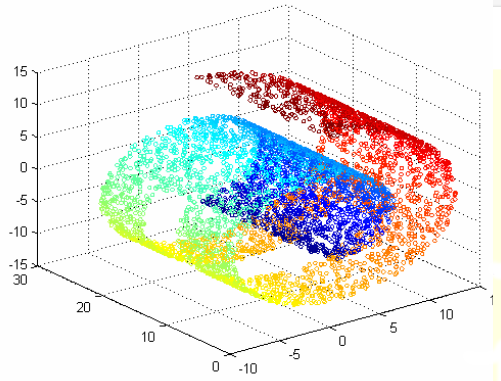
\includegraphics[width=\linewidth]{img/convexity/original.png}
			\captionsetup{justification=centering}
			\caption{The non-convex Swiss-roll.}
		\end{subfigure}
		~
		\begin{subfigure}[H]{.45\linewidth}
			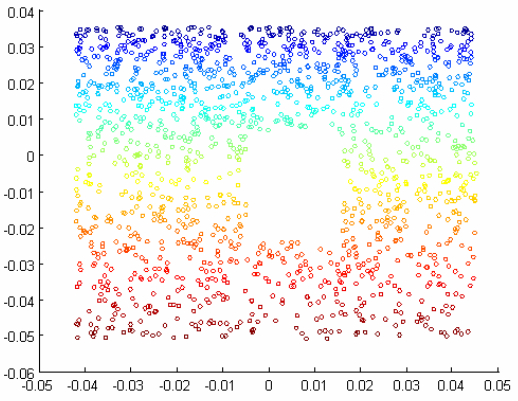
\includegraphics[width=\linewidth]{img/convexity/expected.png}
			\captionsetup{justification=centering}
			\caption{The expected reduction.}
		\end{subfigure}
		\newline\newline
		
		\begin{subfigure}[H]{.45\linewidth}
			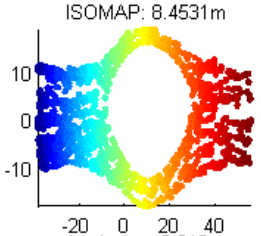
\includegraphics[width=\linewidth]{img/convexity/actual.png}
			\captionsetup{justification=centering}
			\caption{The actual reduction.}
		\end{subfigure}
	\end{figure}
	
	\newpage
	\item[Noise] Noise in data is expressed by samples that somehow diverge from their neighborhood (outliers). As these samples become farthest from its original neighborhood, the chances of being linked to samples from other neighborhood increase, possibly decreasing the quality of the solution. A possible solution is to remove these samples during the pre-processing stage \cite{herik2009}.
	
	The image bellow illustrates an attempt to use Isomap to reduce the $M_{n=.4}$, which is the Swiss-roll data set subjected to a noise factor of $.8$:
	
	\begin{figure}[H]
		\centering
		\begin{subfigure}{.55\linewidth}
			\centering
			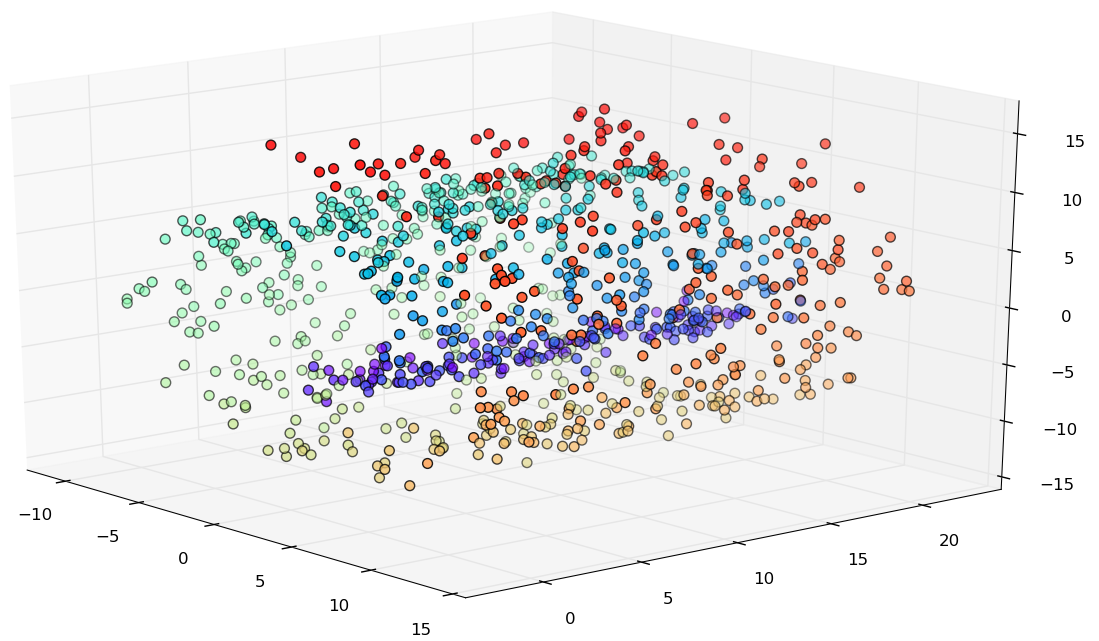
\includegraphics[width=\linewidth]{img/noise/sr/1}
			\captionsetup{justification=centering}
			\caption{The data set $M_{n=.8}$.}
		\end{subfigure}~
		\begin{subfigure}{.45\linewidth}
			\centering
			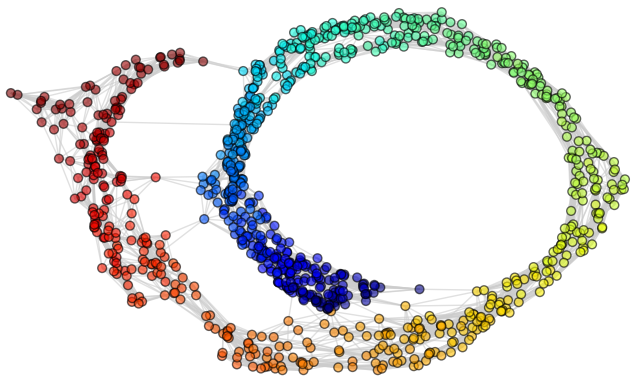
\includegraphics[width=\linewidth]{img/noise/sr/3}
			\captionsetup{justification=centering}
			\caption{The neighborhood graph extracted from $M_{n=.8}$.}
			\label{fig:noise_3}
		\end{subfigure}
		\newline\newline\newline
		\begin{subfigure}{.6\linewidth}
			\centering
			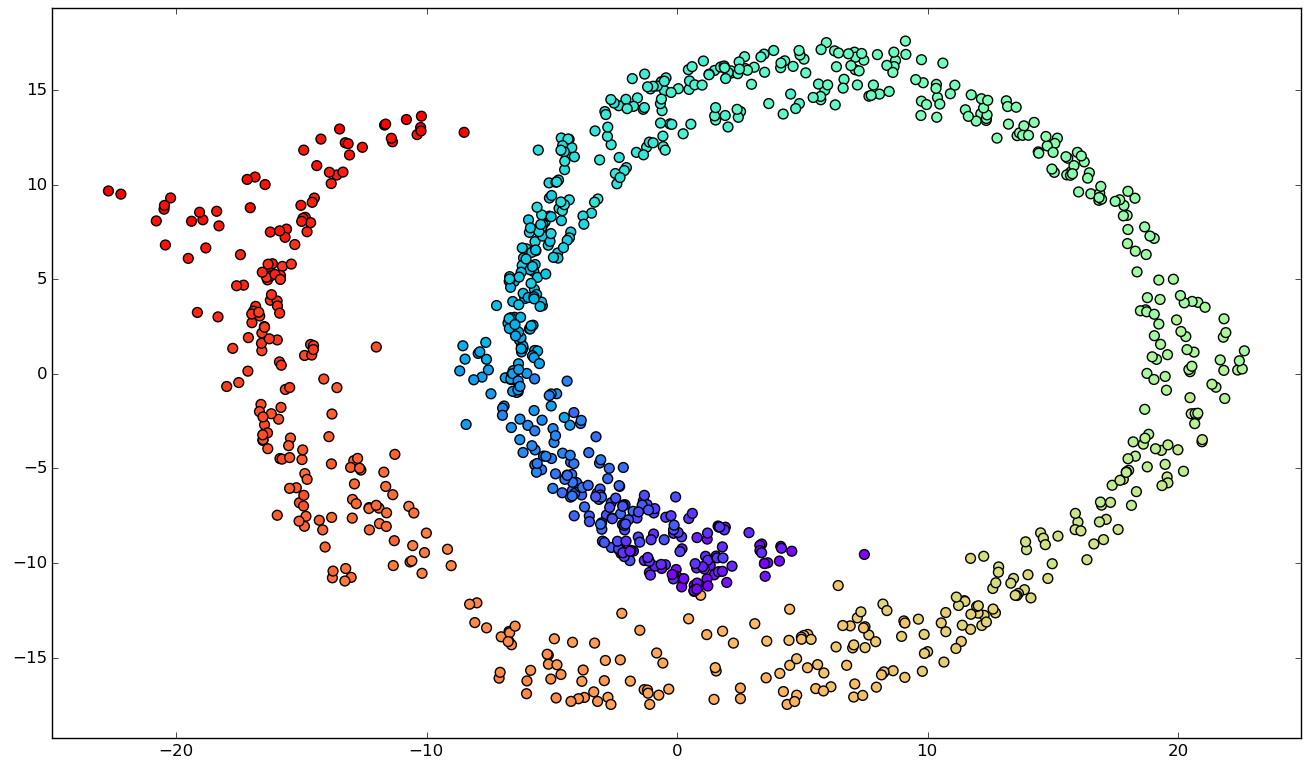
\includegraphics[width=\linewidth]{img/noise/sr/2}
			\captionsetup{justification=centering}
			\caption{$M_{n=.8}$ reduced.}
			\label{fig:noise_2}
		\end{subfigure}
		\captionsetup{justification=centering}
		\caption{The Isomap applied on a noisy data set.}
	\end{figure}
	
	Observe how some outliers were sufficiently far from their original neighborhood in the graph \ref{fig:noise_3}, to the point that Nearest-Neighbor Search maintained the edge between them and samples of completely different colors. MDS then attempted to maintain this dissimilarity, resulting in a deformed reduction (figure \ref{fig:noise_2}).
\end{description}

\subsection{Classification and Regression Over Data Sets Reduced with Isomap}

Just as in \ref{sec:experiments_linear_ds}, this section reports reduction, classification and regression experiments made in common data sets, following the same format as before.

\subsubsection{The Swiss Roll Data Set}

\begin{figure}[H]
	\centering
	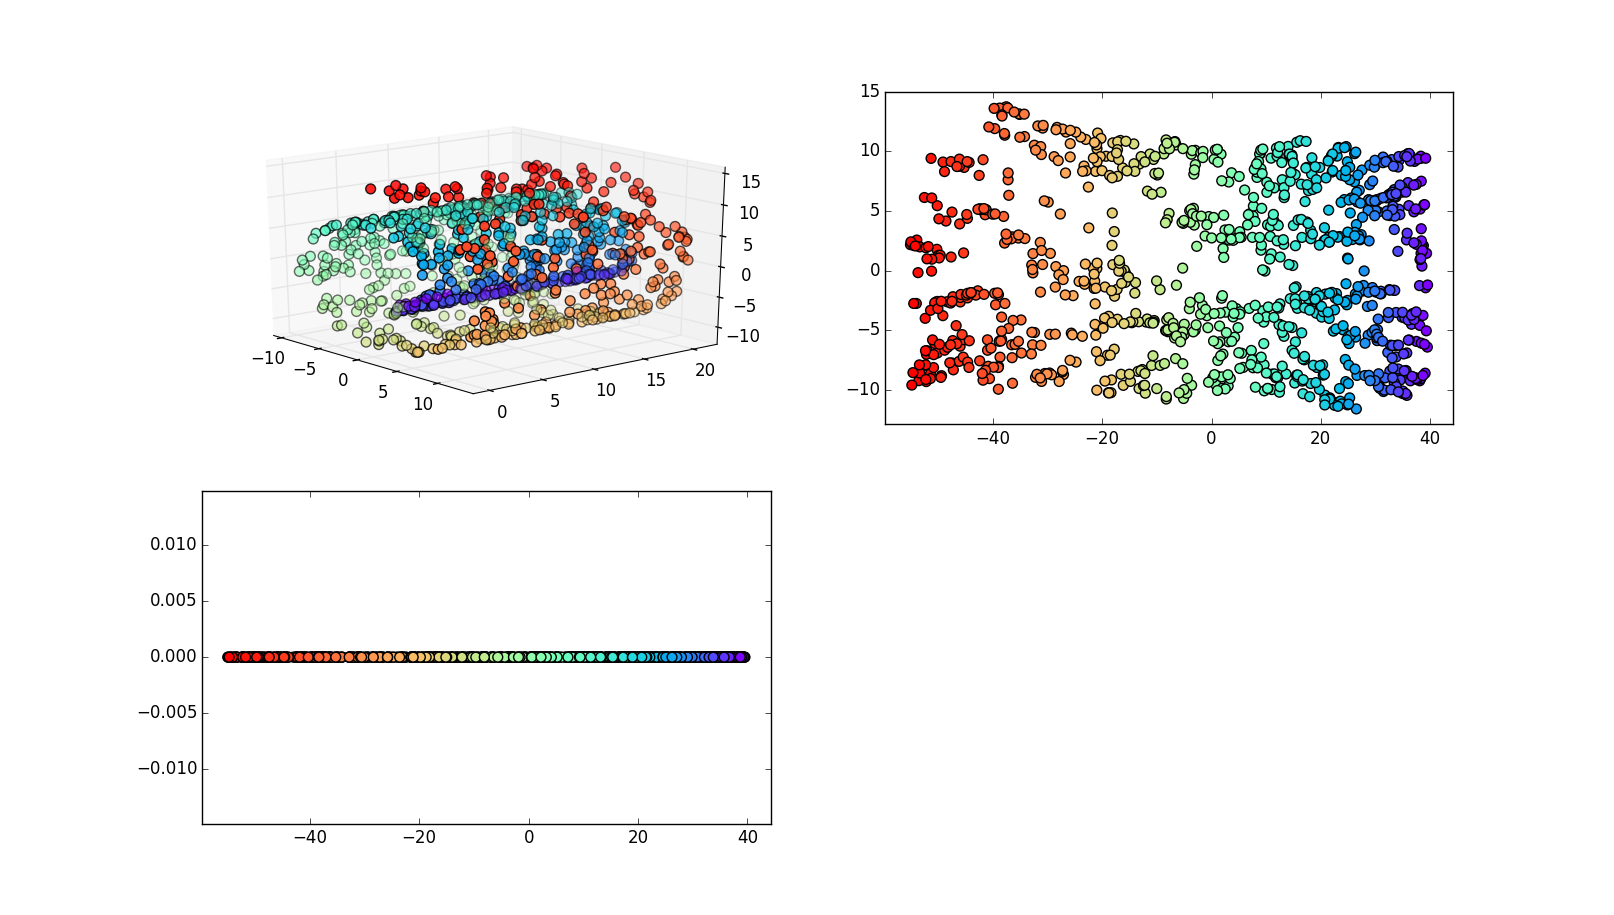
\includegraphics[width=\linewidth]{swiss_isomap}
	\captionsetup{justification=centering}
	\caption{The Swiss Roll data set and its reductions to two and one dimensions, respectively.}
\end{figure}

\begin{table}[H]
	\centering
	\begin{tabular}{|c|c|c|c|}
		\hline
		& \textbf{$\mathbb{R}^3$} & \textbf{$\mathbb{R}^2$} & \textbf{$\mathbb{R}$} \\\hline
		\textbf{Prediction accuracy}   & 1            & 1             & 1     \\\hline
		\textbf{GridSearch time} & 15.53 s   & 415.72 s  & 387.98 s  \\\hline
		\textbf{Reduction time}  & -         & 0.51 s       & 0.48 s     \\\hline
		\textbf{Data size}          & 23.44 KB & 15.62 KB  & 7.81 KB   \\\hline
	\end{tabular}

	\caption{Description of predictions and reduction performance for Swiss Roll.}
\end{table}

\subsubsection{The Digits Data Set}

We will analyze Digits once again, only this time it will be reduced with the Isomap algorithm.

\begin{figure}[H]
	\centering
	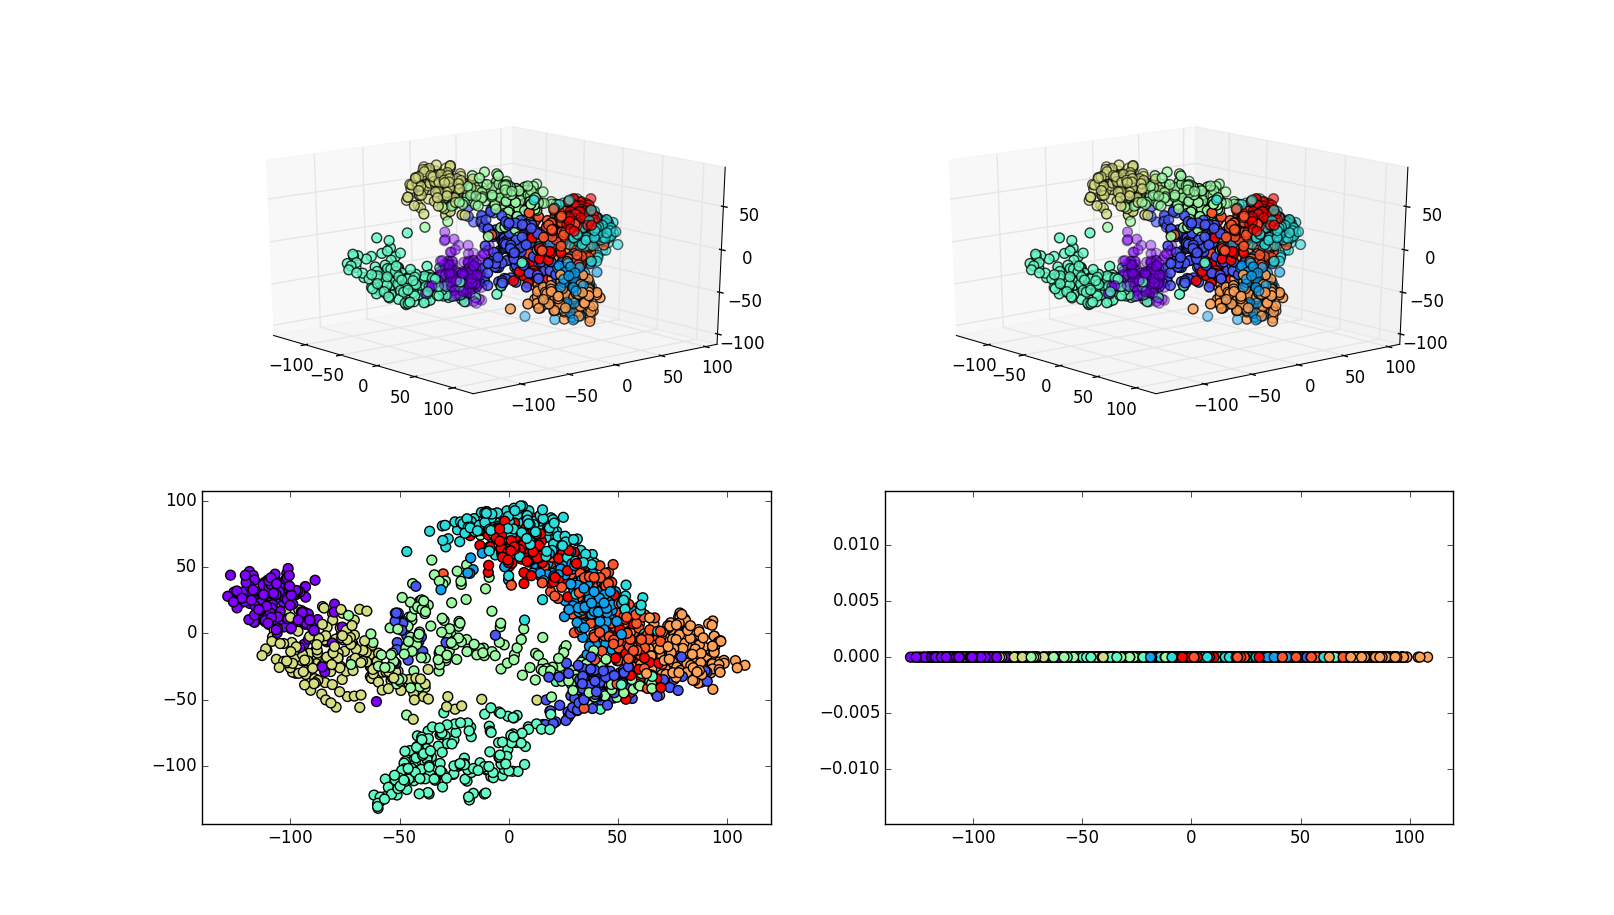
\includegraphics[width=\linewidth]{dsdigitsiso}
	\captionsetup{justification=centering}
	\caption{Digits data set reduced to 10, 3, 2 and 1 dimension, respectively.}
	\label{fig:dsdigitsiso}
\end{figure}

\begin{table}[H]
	\centering
	\begin{tabular}{|c|c|c|c|c|c|}
		\hline
		& \textbf{$\mathbb{R}^{64}$} & \textbf{$\mathbb{R}^{10}$} & \textbf{$\mathbb{R}^3$} & \textbf{$\mathbb{R}^2$} & \textbf{$\mathbb{R}$} \\\hline
		\textbf{Pred. accuracy}   & .98 & .96 & .91 & .69 & .45 \\\hline
		\textbf{GridSearch time} & 12.22 s & 98.08 s & 287.46 s & 630.47 s & 949.88 s \\\hline
		\textbf{Reduction time}  & - & 5.43 s & 2.72 s & 2.71 s & 2.04 s \\\hline
		\textbf{Data size} & 898.50 KB & 140.39 KB & 42.12 KB & 28.08 KB & 14.04 KB \\\hline
	\end{tabular}

	\caption{Description of predictions and reduction performance for Digits.}
\end{table}

Notice that we managed to reduce the data set to only 3 dimensions while maintaining 91\% of accuracy (remember that dimensionality reduction with PCA would reduce accuracy to 74\%). Accuracy loss is still observable when reducing it to two or one dimensions, although it is less intense than losses caused by linear reduction.

\subsubsection{The Leukemia Data Set}

Extracted from \href{http://mldata.com}{mldata}, the Leukemia data set contains 72 samples and 7130 features. The first 7129 features are expression levels of the genes in a given patient. The 7130th feature $t \in \{-1, 1\}$ indicate which of two variants of leukemia is present in the sample (AML, 25 samples, or ALL, 47 samples). \cite{on:duc_ds}

\begin{figure}[H]
	\centering
	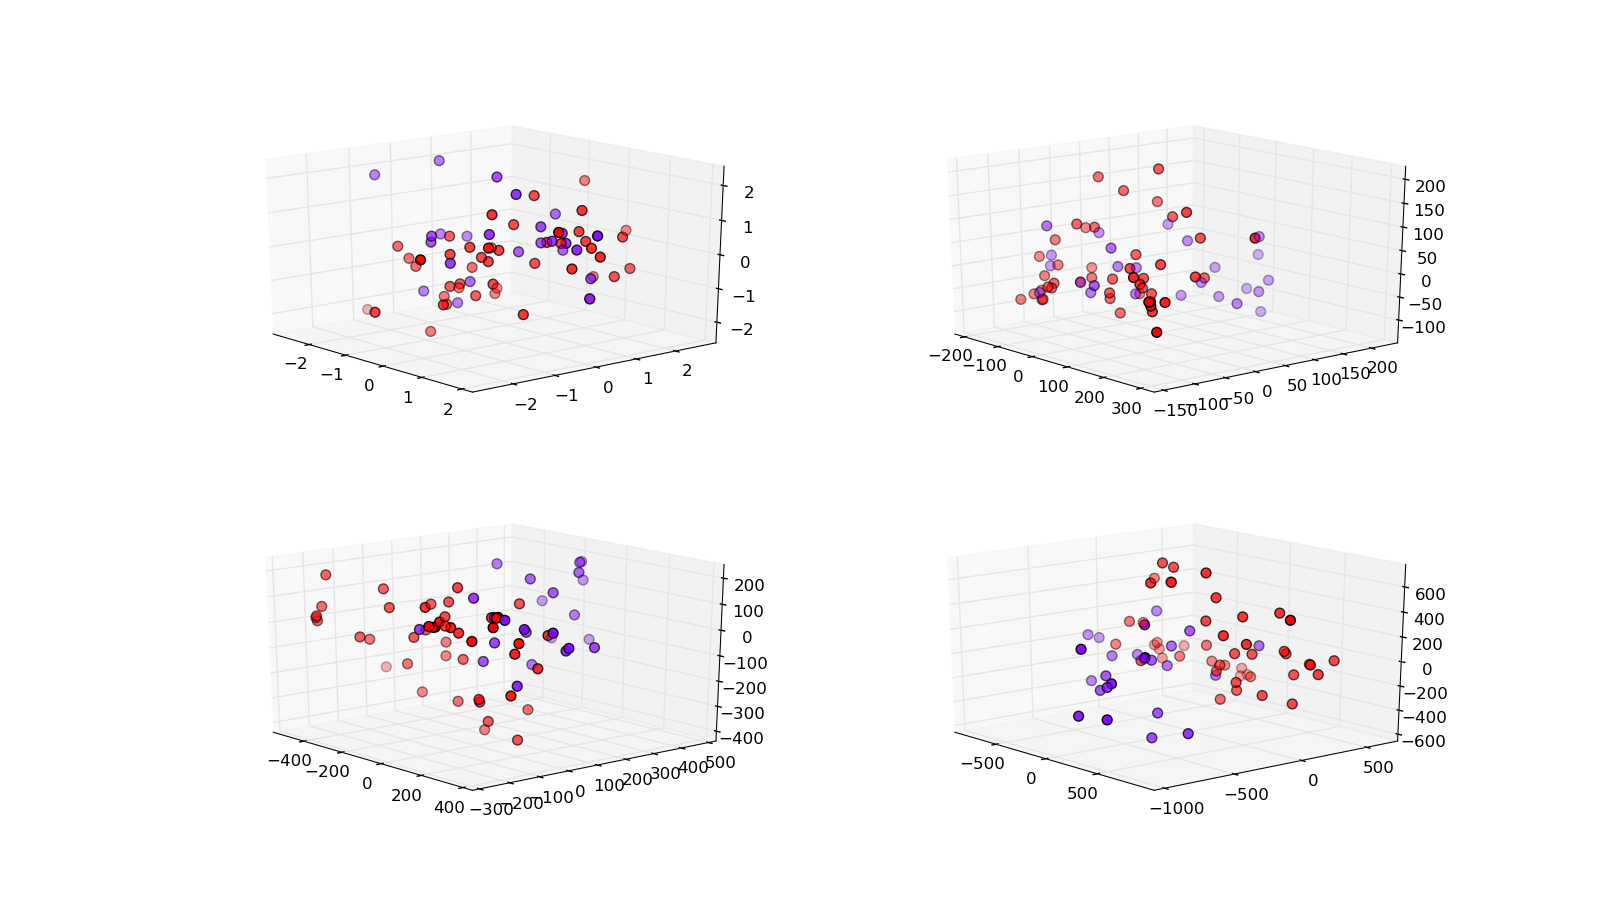
\includegraphics[width=\linewidth]{img/experiments/leukemia}
	\captionsetup{justification=centering}
	\caption{The Leukemia data set and its reduction to 30, 20 and 10 dimensions, respectively.}
	\label{fig:leukemiads}
\end{figure}

\begin{table}[H]
	\centering
	\begin{tabular}{|c|c|c|c|c|}
		\hline
		& \textbf{$\mathbb{R}^{7129}$} & \textbf{$\mathbb{R}^{30}$} & \textbf{$\mathbb{R}^{20}$} & \textbf{$\mathbb{R}^{10}$} \\\hline
		\textbf{Pred. accuracy}    & .99 & .88 & .85 & .88 \\\hline
		\textbf{GridSearch time}   & 2.42 s & .26 s & .26 s & 141.13 s \\\hline
		\textbf{Reduction time}    & - & .06 s & .04 s & .04 s \\\hline
		\textbf{Data size}         & 4010.06 KB & 16.88 KB & 11.25 KB & 5.62 KB \\\hline
	\end{tabular}
	\captionsetup{justification=centering}	
	\caption{Description of predictions and reduction performance for Leukemia data set.}
\end{table}

\newpage
\section{Final Considerations}

% TODO Review this.

In this report, we have approached the subjects of dimensionality reduction. First, focusing on linear methods and their capacity of extract features that maximize variance in a data set, we successfully reduced a limited set of data sets. We then followed to demonstrate how these methods would fail to reduce data sets that followed a nonlinear distribution.

In order to reduce nonlinear data sets, we have introduced the Isomap algorithm, which uses properties commonly present in manifolds (e.g., linear locality, neighborhood). These properties allowed us to map the data sets to an intermediate representation that would only preserve dissimilarities of a restrictive neighborhood that, when given to linear methods, would result in the correct reduction. We then proceeded to formally define Isomap's implementation, and present some of its limitations, variations and applications. Finally, we saw that Isomap can successfully reduce data sets that roughly lie on nonlinear manifolds, but it also strongly dependents on many conditions, such as the manifold assumption, manifold convexity and controlled data noise, severly affecting the number of problems to which it might be applied.

In conclusion, we have observed that although its limitations, Isomap is, indeed, a very regarded method in manifold learning, being cited by many authors since its first presentation and being implemented by many machine learning libraries, in many different languages and environments nowadays.

\newpage

\bibliographystyle{ieeetr}
\bibliography{references}

\end{document}
